\chapter{let's pretend we can read code} 
\label{sec:commentary}
\rhead[]{\leftmark}
\lstset{style=6502Style}
\lstset{ 
   aboveskip=5pt,
   belowskip=0pt,
}
The listing is so short that it possible (and hopefully not too tedious) for us to
review it in its entirety. This will allow us to understand the basic workings of 
a small 'game' such as this one, from booting to running; it will also give us an
accurate idea of how the final 'Psychedelia' product worked. The difference between
the released game and the listing that appeared in Popular Computing Weekly\index{Popular Computing Weekly} is not
qualitative - the underlying structure is the same, the core routines we reviewed 
in the previous chapter are more or less identical. The differences lie only in the
the wealth of options available, so it turns out that the listing is an ideal way
for us to get our heads around the core mechanics of the light synthesizer. In the
chapters that follow we can look at some of the features added to the game in more
detail and concentrate on the individual routines that made them work. Here we will
focus instead on the high-level operation of the game and hopefully obtain a sense
of how the thing hangs together.

For the most part I try to present the code in the order it appears in the game
binary itself, but I have moved some routines around here and there so that we're
reading the code in an order that makes sense to the reader.

Before we drive into the weeds, let's take an aerial view of the code over the next
few pages. This gives us a proper sense of how small the program is and also where
things are in the listing, how it is ordered, and what, if any, structure it possesses.

\subfile{listing_commentary/psychedelia_listing.tex}
\clearpage
\textbf{Lines 46-50. \icode{\textbf{Sys2064}}}
\begin{lstlisting}[caption=The bootstrap routine common to nearly every C64\index{C64} program,escapechar=\%]
* = $0801
;-----------------------------------------------------------------
; Start program at CopyCodeToRAM (SYS 2064)
; SYS 2064 ($0810)
; This is where execution starts.
; It is a short BASIC program that executes whatever is at address
; $0810 (2064 in decimal). In this case, that's CopyCodeToRAM
;-----------------------------------------------------------------
  .BYTE $0B,$08          ; Points to EndOfProgram address below
  .BYTE $0A,$00          ; Arbitrary Line Number, in this case: 0010
  .BYTE $9E              ; SYS
  .BYTE $32,$30,$36,$34  ; 2064 ($810), which is CopyCodeToRAM below.
  .BYTE $00              ; Null byte to terminate the line above.
  .BYTE $00,$00          ; EndOfProgram  (all zeroes)
  .BYTE $00,$00,$00      ; Filler bytes so that InitializeProgram%\index{InitializeProgram}% is
                         ; located at $0810
\end{lstlisting}

\textbf{Lines 56-75. \icode{\textbf{CopyCodeToRam}}}
\begin{lstlisting}[caption=Some strictly unnecessary code copying,escapechar=\%]
RAM0835LoPtr                        = $FD
RAM0835HiPtr                        = $FE
RAM4000HiPtr                        = $FC
RAM4000LoPtr                        = $FB
;---------------------------------------------------
; CopyCodeToRAM
;----------------------------------------------------
CopyCodeToRAM
        LDA #$40
        STA RAM4000HiPtr
        LDA #$08
        STA RAM0835HiPtr
        LDA #$00
        STA RAM4000LoPtr
        LDA #$35
        STA RAM0835LoPtr
        LDY #$00                                 
        LDX #$06
CopyLoop   
        LDA (RAM0835LoPtr),Y
        STA (RAM4000LoPtr),Y
        DEY 
        BNE CopyLoop
        INC RAM4000HiPtr
        INC RAM0835HiPtr
        DEX 
        BNE CopyLoop

        JMP InitializeProgram%\index{InitializeProgram}%

\end{lstlisting}
\clearpage
\rhead[]{launching the game}
\textbf{Lines 46-50. \icode{\textbf{Sys2064}}:} Yay, let's do some admin like starting the program! All C64\index{C64} programs 
begin execution at position \icode{\$0801}, it's the law.
So every C64\index{C64} program has a little section like this that the C64\index{C64} executes first and which tells the C64\index{C64} what to do next.
Here we tell it to start execution at another location \icode{\$0810}. Since we're currently at location \icode{\$0801}, that's
almost 16 bytes ahead and contains the code we've labelled \icode{CopyCodeToRAM} which we jump to next.

The command is given in a slightly strange way. Not strange for the time, but an oddly convoluted convention in its own right.
The \icode{SYS} command is followed by a series of PETSCII values forming the decimal number 2064. In hexadecimal this is
\icode{\$0810} which is the actual location to start executing. So \icode{SYS 2064} as given by '\icode{\$9E, \$32, \$30, \$36,\$34}'
means 'start executing whatever is at memory location \icode{\$0810}'. Which in this case is the little routine \icode{CopyCodeToRAM}.

The 'Abitrary Line Number', is just that: completely arbitrary. Here we have '0010', but in the commercial release of Psychedelia
the value chosen is \icode{\$C1,\$07} - translated to decimal this is '1985', the year of the game's release.

\bigskip
\bigskip
\textbf{Lines 56-75. \icode{\textbf{CopyCodeToRam}}:} Little Commodore 64 programs sure do like copying things around. This routine copies the entire code of the program to a
completely new position in memory at location \icode{\$4000} and then jumps to the routine \icode{InitializeProgram\index{InitializeProgram}} that will actually start running
'Psychedelia'.

I think this was some sort of cheap and dirty copy protection, designed to prevent people from casually disassembling the
program if they felt minded to do so. 
\bigskip
\begin{definition2}[Friendly Blue Learning Box]
\setlength{\intextsep}{0pt}%
\setlength{\columnsep}{3pt}%
\begin{wrapfigure}{l}{0.48\textwidth}
  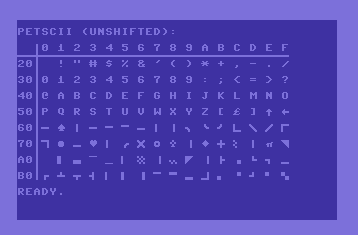
\includegraphics[width=6cm]{src/listing_commentary/petscii.png}
\end{wrapfigure}
\small
PETSCII is the Commodore 64's flavour of the ASCII character set. It is simply a convention that attributes certain byte
values to certain characters and numbers. For example, the value \icode{\$41} signifies the \icode{A} character, \icode{\$42}
signifies the \icode{B} character. Likewise \icode{\$31} signifies the numeral \icode{1}, \icode{\$32} the numeral \icode{2},
and so on. These values are arbitrary, so purely conventional. It is possible for the programmer to use customized values
and map them to any character set they please.
\end{definition2}

\clearpage
\textbf{Lines 82-113. \icode{\textbf{InitializeProgram\index{InitializeProgram}}}}
\begin{lstlisting}[caption=The initialization routine - visited only once\, at the very start of execution,escapechar=\%]
NUM_COLS  = $28
NUM_ROWS  = $18
COLOR_RAM = $D800
;-------------------------------------------------------
; InitializeProgram%\index{InitializeProgram}%
;-------------------------------------------------------
InitializeProgram%\index{InitializeProgram}%   
        LDA #BLACK
        STA $D020    ;Border Color
        STA $D021    ;Background Color 0

PrepareHiLoPtrs
        LDA #>COLOR_RAM
        STA colorRamHiPtr%\index{colorRamHiPtr}%
        LDA #<COLOR_RAM
        STA colorRamLoPtr%\index{colorRamLoPtr}%

        LDX #$00
FillLinePointerLoop
        LDA colorRamHiPtr%\index{colorRamHiPtr}%
        STA colorRAMLineTableHiPtrArray%\index{colorRAMLineTableHiPtrArray}%,X
        LDA colorRamLoPtr%\index{colorRamLoPtr}%
        STA colorRAMLineTableLoPtrArray%\index{colorRAMLineTableLoPtrArray}%,X
        CLC 
        ADC #NUM_COLS
        STA colorRamLoPtr%\index{colorRamLoPtr}%
        LDA colorRamHiPtr%\index{colorRamHiPtr}%
        ADC #$00
        STA colorRamHiPtr%\index{colorRamHiPtr}%
        INX 
        CPX #NUM_ROWS+1
        BNE FillLinePointerLoop

        JSR InitializeScreenAndText
        JMP LaunchPsychedelia%\index{LaunchPsychedelia}%

\end{lstlisting}
\clearpage

\rhead[]{\icode{InitializeProgram\index{InitializeProgram}}}
\textbf{Lines 82-113. \icode{\textbf{InitializeProgram\index{InitializeProgram}}}:} More admin!  First we set the background and border color to black by loading
\icode{\$00} to the memory locations \icode{\$D020} for the border and \icode{\$D021} for the background color.

\bigskip
\bigskip
\textbf{Lines 90-93. \icode{\textbf{PrepareHiLoPtrs}}:} \icode{COLOR\_RAM} (\icode{\$D800}) is the address at which Color RAM starts. Color
RAM is a region of memory 1000 bytes long that contains the color value for each of the 25 rows of 40 characters that get displayed on the
screen. 

In order to be able to work with this address we need to have a way of working with values that are two bytes long even though
our 6502 instruction set only accomodates single byte values. To do this we have to split the address in two and store each half in 
a separate variable. \icode{LDA \#>COLOR\_RAM} is an assembly language convention for referencing the first byte in the two byte address
\icode{COLOR\_RAM}, i.e \icode{\$D800}. So another way of writing it is simply: \icode{LDA \#\$D8}. Likewise \icode{LDA \#<COLOR\_RAM} is
another way of writing \icode{LDA \#\$00}. 

We're storing each of these values in \icode{colorRamHiPtr\index{colorRamHiPtr}} and \icode{colorRamLoPtr\index{colorRamLoPtr}} respectively
as we're going to use them to populate a pair of arrays with each half of the addresses of each of the 25 rows on the screen.


\bigskip
\bigskip
\textbf{Lines 101-113. \textbf{\icode{FillLinePointerLoop}}:} Here we set up the pair of arrays that Psychedelia will make heavy use of:
\icode{colorRAMLineTableHiPtrArray\index{colorRAMLineTableHiPtrArray}} and \icode{colorRAMLineTable\-LoPtrArray}.
Together these arrays will function as a map on to the screen for drawing our pixels. Since the Commodore 64 screen is 25 rows high we make each array
25 elements long and together each element in each array will combine to give the address on the screen for the start of each row.
\begin{figure}[H]
  {
    \setlength{\tabcolsep}{3.0pt}
    \setlength\cmidrulewidth{\heavyrulewidth} % Make cmidrule = 
    \begin{adjustbox}{width=8cm,center}
      \begin{tabular}{cccc}
        \toprule
        Element &
        \makecell[c]{\icode{colorRAMLineTable} \\ \icode{HiPtrArray}} & 
        \makecell[c]{\icode{colorRAMLineTable} \\ \icode{LoPtrArray}} & 
        Address \\
        \midrule
0 & \icode{\$D8} & \icode{\$00} & \icode{\$D800} \\ 
1 & \icode{\$D8} & \icode{\$28} & \icode{\$D828} \\ 
. & . & . & .\\
6 & \icode{\$D8} & \icode{\$F0} & \icode{\$D8F0} \\ 
. & . & . & .\\
23 & \icode{\$DB} & \icode{\$70} & \icode{\$DB70} \\ 
24 & \icode{\$DB} & \icode{\$98} & \icode{\$DB98} \\ 
        \bottomrule
      \end{tabular}
    \end{adjustbox}
  }\caption{Our two arrays and their contents - each combining to give us an address for the start of each row in Color RAM. }
\end{figure}

So in practice what this gives us is a 'single array' with which we can address each row on the screen and write color values
to the pixel position of our choice.


\begin{figure}[H]
  {
    \setlength{\tabcolsep}{3.0pt}
    \setlength\cmidrulewidth{\heavyrulewidth} % Make cmidrule = 
    \begin{adjustbox}{width=12cm,center}
      \begin{tabular}{cc}
        \toprule
        Color Ram Address & Color RAM Bytes \\
        \midrule
\icode{\$D800} & \makecell[l]{\icode{00}  \icode{00}  \icode{00}  \icode{00}  \icode{00}  \icode{00}  \icode{00}  \icode{00}  \icode{00}  \icode{00}  \icode{00}  \icode{00}  \icode{00}  \icode{00}  \icode{00}  \icode{00}  \icode{00}  \icode{00}  \icode{00}  \icode{00}  \icode{00}  \icode{00}  \icode{00}  \icode{00}  \icode{00}  \icode{00}  \icode{00}  \icode{00}  \icode{00}  \icode{00}  \icode{00}  \icode{00}  \icode{00}  \icode{00}  \icode{00}  \icode{00}  \icode{00}  \icode{00}  \icode{00}  \icode{00}   \\}\\
\icode{\$D828} & \makecell[l]{\icode{00}  \icode{00}  \icode{00}  \icode{00}  \icode{00}  \icode{00}  \icode{00}  \icode{00}  \icode{00}  \icode{00}  \icode{00}  \icode{00}  \icode{00}  \icode{00}  \icode{00}  \icode{00}  \icode{00}  \icode{00}  \icode{00}  \icode{00}  \icode{00}  \icode{00}  \icode{00}  \icode{00}  \icode{00}  \icode{00}  \icode{00}  \icode{00}  \icode{00}  \icode{00}  \icode{00}  \icode{00}  \icode{00}  \icode{00}  \icode{00}  \icode{00}  \icode{00}  \icode{00}  \icode{00}  \icode{00}   \\}\\
\icode{\$D850} & \makecell[l]{\icode{00}  \icode{00}  \icode{00}  \icode{00}  \icode{00}  \icode{00}  \icode{00}  \icode{00}  \icode{00}  \icode{00}  \icode{00}  \icode{00}  \icode{00}  \icode{00}  \icode{00}  \icode{00}  \icode{00}  \icode{00}  \icode{00}  \icode{00}  \icode{00}  \icode{00}  \icode{00}  \icode{00}  \icode{00}  \icode{00}  \icode{00}  \icode{00}  \icode{00}  \icode{00}  \icode{00}  \icode{00}  \icode{00}  \icode{00}  \icode{00}  \icode{00}  \icode{00}  \icode{00}  \icode{00}  \icode{00}   \\}\\
\icode{\$D878} & \makecell[l]{\icode{00}  \icode{00}  \icode{00}  \icode{00}  \icode{00}  \icode{00}  \icode{00}  \icode{00}  \icode{00}  \icode{00}  \icode{00}  \icode{00}  \icode{00}  \icode{00}  \icode{00}  \icode{00}  \icode{00}  \icode{00}  \icode{00}  \icode{00}  \icode{00}  \icode{00}  \icode{00}  \icode{00}  \icode{00}  \icode{00}  \icode{00}  \icode{00}  \icode{00}  \icode{00}  \icode{00}  \icode{00}  \icode{00}  \icode{00}  \icode{00}  \icode{00}  \icode{00}  \icode{00}  \icode{00}  \icode{00}   \\}\\
\icode{\$D8A0} & \makecell[l]{\icode{00}  \icode{00}  \icode{00}  \icode{00}  \icode{00}  \icode{00}  \icode{00}  \icode{00}  \icode{00}  \icode{00}  \icode{00}  \icode{00}  \icode{00}  \icode{00}  \icode{00}  \icode{00}  \icode{00}  \icode{00}  \icode{00}  \icode{00}  \icode{00}  \icode{00}  \icode{00}  \icode{00}  \icode{00}  \icode{00}  \icode{00}  \icode{00}  \icode{00}  \icode{00}  \icode{00}  \icode{00}  \icode{00}  \icode{00}  \icode{00}  \icode{00}  \icode{00}  \icode{00}  \icode{00}  \icode{00}   \\}\\
\icode{\$D8C8} & \makecell[l]{\icode{00}  \icode{00}  \icode{00}  \icode{00}  \icode{00}  \icode{00}  \icode{00}  \icode{00}  \icode{00}  \icode{00}  \icode{00}  \icode{00}  \icode{00}  \icode{00}  \icode{00}  \icode{00}  \icode{00}  \icode{00}  \icode{00}  \icode{00}  \icode{00}  \icode{00}  \icode{00}  \icode{00}  \icode{00}  \icode{00}  \icode{00}  \icode{00}  \icode{00}  \icode{00}  \icode{00}  \icode{00}  \icode{00}  \icode{00}  \icode{00}  \icode{00}  \icode{00}  \icode{00}  \icode{00}  \icode{00}   \\}\\
\icode{\$D8F0} & \makecell[l]{\icode{00}  \icode{00}  \icode{00}  \icode{00}  \icode{00}  \icode{00}  \icode{00}  \icode{00}  \icode{00}  \icode{00}  \icode{00}  \icode{00}  \icode{00}  \icode{00}  \icode{00}  \icode{00}  \icode{00}  \textcolor{red}{\icode{02}}  \icode{00}  \textcolor{red}{\icode{02}}  \icode{00}  \icode{00}  \icode{00}  \icode{00}  \icode{00}  \icode{00}  \icode{00}  \icode{00}  \icode{00}  \icode{00}  \icode{00}  \icode{00}  \icode{00}  \icode{00}  \icode{00}  \icode{00}  \icode{00}  \icode{00}  \icode{00}  \icode{00}   \\}\\
\icode{\$D918} & \makecell[l]{\icode{00}  \icode{00}  \icode{00}  \icode{00}  \icode{00}  \icode{00}  \icode{00}  \icode{00}  \icode{00}  \icode{00}  \icode{00}  \icode{00}  \icode{00}  \icode{00}  \icode{00}  \icode{00}  \icode{00}  \icode{00}  \textcolor{red}{\icode{02}}  \icode{00}  \icode{00}  \icode{00}  \icode{00}  \icode{00}  \icode{00}  \icode{00}  \icode{00}  \icode{00}  \icode{00}  \icode{00}  \icode{00}  \icode{00}  \icode{00}  \icode{00}  \icode{00}  \icode{00}  \icode{00}  \icode{00}  \icode{00}  \icode{00}   \\}\\
\icode{\$D940} & \makecell[l]{\icode{00}  \icode{00}  \icode{00}  \icode{00}  \icode{00}  \icode{00}  \icode{00}  \icode{00}  \icode{00}  \icode{00}  \icode{00}  \icode{00}  \icode{00}  \icode{00}  \icode{00}  \icode{00}  \icode{00}  \icode{00}  \textcolor{green}{\icode{05}}  \icode{00}  \icode{00}  \icode{00}  \icode{00}  \icode{00}  \icode{00}  \icode{00}  \icode{00}  \icode{00}  \icode{00}  \icode{00}  \icode{00}  \icode{00}  \icode{00}  \icode{00}  \icode{00}  \icode{00}  \icode{00}  \icode{00}  \icode{00}  \icode{00}   \\}\\
\icode{\$D968} & \makecell[l]{\icode{00}  \icode{00}  \icode{00}  \icode{00}  \icode{00}  \icode{00}  \icode{00}  \icode{00}  \icode{00}  \icode{00}  \icode{00}  \icode{00}  \icode{00}  \icode{00}  \icode{00}  \icode{00}  \icode{00}  \icode{00}  \textcolor{cyan}{\icode{03}}  \icode{00}  \icode{00}  \icode{00}  \icode{00}  \icode{00}  \icode{00}  \icode{00}  \icode{00}  \icode{00}  \icode{00}  \icode{00}  \icode{00}  \icode{00}  \icode{00}  \icode{00}  \icode{00}  \icode{00}  \icode{00}  \icode{00}  \icode{00}  \icode{00}   \\}\\
\icode{\$D990} & \makecell[l]{\icode{00}  \icode{00}  \icode{00}  \icode{00}  \icode{00}  \icode{00}  \icode{00}  \icode{00}  \icode{00}  \icode{00}  \icode{00}  \icode{00}  \icode{00}  \textcolor{red}{\icode{02}}  \icode{00}  \icode{00}  \icode{00}  \textcolor{yellow}{\icode{07}}  \textcolor{yellow}{\icode{07}}  \textcolor{yellow}{\icode{07}}  \icode{00}  \icode{00}  \icode{00}  \textcolor{red}{\icode{02}}  \icode{00}  \icode{00}  \icode{00}  \icode{00}  \icode{00}  \icode{00}  \icode{00}  \icode{00}  \icode{00}  \icode{00}  \icode{00}  \icode{00}  \icode{00}  \icode{00}  \icode{00}  \icode{00}   \\}\\
\icode{\$D9B8} & \makecell[l]{\icode{00}  \icode{00}  \icode{00}  \icode{00}  \icode{00}  \icode{00}  \icode{00}  \icode{00}  \icode{00}  \icode{00}  \icode{00}  \icode{00}  \icode{00}  \icode{00}  \textcolor{red}{\icode{02}}  \textcolor{green}{\icode{05}}  \textcolor{cyan}{\icode{03}}  \textcolor{yellow}{\icode{07}}  \textcolor{yellow}{\icode{07}}  \textcolor{yellow}{\icode{07}}  \textcolor{cyan}{\icode{03}}  \textcolor{green}{\icode{05}}  \textcolor{red}{\icode{02}}  \icode{00}  \icode{00}  \icode{00}  \icode{00}  \icode{00}  \icode{00}  \icode{00}  \icode{00}  \icode{00}  \icode{00}  \icode{00}  \icode{00}  \icode{00}  \icode{00}  \icode{00}  \icode{00}  \icode{00}   \\}\\
\icode{\$D9E0} & \makecell[l]{\icode{00}  \icode{00}  \icode{00}  \icode{00}  \icode{00}  \icode{00}  \icode{00}  \icode{00}  \icode{00}  \icode{00}  \icode{00}  \icode{00}  \icode{00}  \textcolor{red}{\icode{02}}  \icode{00}  \icode{00}  \icode{00}  \textcolor{yellow}{\icode{07}}  \textcolor{yellow}{\icode{07}}  \textcolor{yellow}{\icode{07}}  \icode{00}  \icode{00}  \icode{00}  \textcolor{red}{\icode{02}}  \icode{00}  \icode{00}  \icode{00}  \icode{00}  \icode{00}  \icode{00}  \icode{00}  \icode{00}  \icode{00}  \icode{00}  \icode{00}  \icode{00}  \icode{00}  \icode{00}  \icode{00}  \icode{00}   \\}\\
\icode{\$DA08} & \makecell[l]{\icode{00}  \icode{00}  \icode{00}  \icode{00}  \icode{00}  \icode{00}  \icode{00}  \icode{00}  \icode{00}  \icode{00}  \icode{00}  \icode{00}  \icode{00}  \icode{00}  \icode{00}  \icode{00}  \icode{00}  \icode{00}  \textcolor{cyan}{\icode{03}}  \icode{00}  \icode{00}  \icode{00}  \icode{00}  \icode{00}  \icode{00}  \icode{00}  \icode{00}  \icode{00}  \icode{00}  \icode{00}  \icode{00}  \icode{00}  \icode{00}  \icode{00}  \icode{00}  \icode{00}  \icode{00}  \icode{00}  \icode{00}  \icode{00}   \\}\\
\icode{\$DA30} & \makecell[l]{\icode{00}  \icode{00}  \icode{00}  \icode{00}  \icode{00}  \icode{00}  \icode{00}  \icode{00}  \icode{00}  \icode{00}  \icode{00}  \icode{00}  \icode{00}  \icode{00}  \icode{00}  \icode{00}  \icode{00}  \icode{00}  \textcolor{green}{\icode{05}}  \icode{00}  \icode{00}  \icode{00}  \icode{00}  \icode{00}  \icode{00}  \icode{00}  \icode{00}  \icode{00}  \icode{00}  \icode{00}  \icode{00}  \icode{00}  \icode{00}  \icode{00}  \icode{00}  \icode{00}  \icode{00}  \icode{00}  \icode{00}  \icode{00}   \\}\\
\icode{\$DA58} & \makecell[l]{\icode{00}  \icode{00}  \icode{00}  \icode{00}  \icode{00}  \icode{00}  \icode{00}  \icode{00}  \icode{00}  \icode{00}  \icode{00}  \icode{00}  \icode{00}  \icode{00}  \icode{00}  \icode{00}  \icode{00}  \icode{00}  \textcolor{red}{\icode{02}}  \icode{00}  \icode{00}  \icode{00}  \icode{00}  \icode{00}  \icode{00}  \icode{00}  \icode{00}  \icode{00}  \icode{00}  \icode{00}  \icode{00}  \icode{00}  \icode{00}  \icode{00}  \icode{00}  \icode{00}  \icode{00}  \icode{00}  \icode{00}  \icode{00}   \\}\\
\icode{\$DA80} & \makecell[l]{\icode{00}  \icode{00}  \icode{00}  \icode{00}  \icode{00}  \icode{00}  \icode{00}  \icode{00}  \icode{00}  \icode{00}  \icode{00}  \icode{00}  \icode{00}  \icode{00}  \icode{00}  \icode{00}  \icode{00}  \textcolor{red}{\icode{02}}  \icode{00}  \textcolor{red}{\icode{02}}  \icode{00}  \icode{00}  \icode{00}  \icode{00}  \icode{00}  \icode{00}  \icode{00}  \icode{00}  \icode{00}  \icode{00}  \icode{00}  \icode{00}  \icode{00}  \icode{00}  \icode{00}  \icode{00}  \icode{00}  \icode{00}  \icode{00}  \icode{00}   \\}\\
\icode{\$DAA8} & \makecell[l]{\icode{00}  \icode{00}  \icode{00}  \icode{00}  \icode{00}  \icode{00}  \icode{00}  \icode{00}  \icode{00}  \icode{00}  \icode{00}  \icode{00}  \icode{00}  \icode{00}  \icode{00}  \icode{00}  \icode{00}  \icode{00}  \icode{00}  \icode{00}  \icode{00}  \icode{00}  \icode{00}  \icode{00}  \icode{00}  \icode{00}  \icode{00}  \icode{00}  \icode{00}  \icode{00}  \icode{00}  \icode{00}  \icode{00}  \icode{00}  \icode{00}  \icode{00}  \icode{00}  \icode{00}  \icode{00}  \icode{00}   \\}\\
\icode{\$DAD0} & \makecell[l]{\icode{00}  \icode{00}  \icode{00}  \icode{00}  \icode{00}  \icode{00}  \icode{00}  \icode{00}  \icode{00}  \icode{00}  \icode{00}  \icode{00}  \icode{00}  \icode{00}  \icode{00}  \icode{00}  \icode{00}  \icode{00}  \icode{00}  \icode{00}  \icode{00}  \icode{00}  \icode{00}  \icode{00}  \icode{00}  \icode{00}  \icode{00}  \icode{00}  \icode{00}  \icode{00}  \icode{00}  \icode{00}  \icode{00}  \icode{00}  \icode{00}  \icode{00}  \icode{00}  \icode{00}  \icode{00}  \icode{00}   \\}\\
\icode{\$DAF8} & \makecell[l]{\icode{00}  \icode{00}  \icode{00}  \icode{00}  \icode{00}  \icode{00}  \icode{00}  \icode{00}  \icode{00}  \icode{00}  \icode{00}  \icode{00}  \icode{00}  \icode{00}  \icode{00}  \icode{00}  \icode{00}  \icode{00}  \icode{00}  \icode{00}  \icode{00}  \icode{00}  \icode{00}  \icode{00}  \icode{00}  \icode{00}  \icode{00}  \icode{00}  \icode{00}  \icode{00}  \icode{00}  \icode{00}  \icode{00}  \icode{00}  \icode{00}  \icode{00}  \icode{00}  \icode{00}  \icode{00}  \icode{00}   \\}\\
\icode{\$DB20} & \makecell[l]{\icode{00}  \icode{00}  \icode{00}  \icode{00}  \icode{00}  \icode{00}  \icode{00}  \icode{00}  \icode{00}  \icode{00}  \icode{00}  \icode{00}  \icode{00}  \icode{00}  \icode{00}  \icode{00}  \icode{00}  \icode{00}  \icode{00}  \icode{00}  \icode{00}  \icode{00}  \icode{00}  \icode{00}  \icode{00}  \icode{00}  \icode{00}  \icode{00}  \icode{00}  \icode{00}  \icode{00}  \icode{00}  \icode{00}  \icode{00}  \icode{00}  \icode{00}  \icode{00}  \icode{00}  \icode{00}  \icode{00}   \\}\\
\icode{\$DB48} & \makecell[l]{\icode{00}  \icode{00}  \icode{00}  \icode{00}  \icode{00}  \icode{00}  \icode{00}  \icode{00}  \icode{00}  \icode{00}  \icode{00}  \icode{00}  \icode{00}  \icode{00}  \icode{00}  \icode{00}  \icode{00}  \icode{00}  \icode{00}  \icode{00}  \icode{00}  \icode{00}  \icode{00}  \icode{00}  \icode{00}  \icode{00}  \icode{00}  \icode{00}  \icode{00}  \icode{00}  \icode{00}  \icode{00}  \icode{00}  \icode{00}  \icode{00}  \icode{00}  \icode{00}  \icode{00}  \icode{00}  \icode{00}   \\}\\
\icode{\$DB70} & \makecell[l]{\icode{00}  \icode{00}  \icode{00}  \icode{00}  \icode{00}  \icode{00}  \icode{00}  \icode{00}  \icode{00}  \icode{00}  \icode{00}  \icode{00}  \icode{00}  \icode{00}  \icode{00}  \icode{00}  \icode{00}  \icode{00}  \icode{00}  \icode{00}  \icode{00}  \icode{00}  \icode{00}  \icode{00}  \icode{00}  \icode{00}  \icode{00}  \icode{00}  \icode{00}  \icode{00}  \icode{00}  \icode{00}  \icode{00}  \icode{00}  \icode{00}  \icode{00}  \icode{00}  \icode{00}  \icode{00}  \icode{00}   \\}\\
\icode{\$DB98} & \makecell[l]{\icode{00}  \icode{00}  \icode{00}  \icode{00}  \icode{00}  \icode{00}  \icode{00}  \icode{00}  \icode{00}  \icode{00}  \icode{00}  \icode{00}  \icode{00}  \icode{00}  \icode{00}  \icode{00}  \icode{00}  \icode{00}  \icode{00}  \icode{00}  \icode{00}  \icode{00}  \icode{00}  \icode{00}  \icode{00}  \icode{00}  \icode{00}  \icode{00}  \icode{00}  \icode{00}  \icode{00}  \icode{00}  \icode{00}  \icode{00}  \icode{00}  \icode{00}  \icode{00}  \icode{00}  \icode{00}  \icode{00}   \\}\\
        \bottomrule
      \end{tabular}
    \end{adjustbox}
  }\caption{Color RAM for the screen with the starting address for each row on the left. }
\end{figure}



For example, to make the pixel on row 7 and column 15 red above, we have written a value of \icode{02} to the address \icode{\$D8FF}. This 
address is
formed from adding \icode{\$D8F0} (the 7th element in our array) + 15, i.e. \icode{\$D8F0} + \icode{\$0F} = \icode{\$D8FF}. 
To actually do this we would do something like the following:
 
\begin{lstlisting}[escapechar=\%]
    RED = $02
    ; Load the 7th element from each array.
    LDX #$06
    ; This stores $F0 in currentLineInColorRamLoPtr
    LDA colorRAMLineTableLoPtrArray%\index{colorRAMLineTableLoPtrArray}%,X
    STA currentLineInColorRamLoPtr
    ; This stores $D8 in currentLineInColorRamHiPtr
    LDA colorRAMLineTableHiPtrArray%\index{colorRAMLineTableHiPtrArray}%,X
    STA currentLineInColorRamHiPtr
    ; Load $02, i.e. RED, to the Accumulator. 
    LDA #RED
    ; Y will be our index so give it the offset into the
    ; line, i.e. 15. 
    LDY #$0F
    ; Write $02 to address $DBFF, painting it red.
    STA (currentLineInColorRamLoPtr),Y
\end{lstlisting}

This gives us an idea of how the array will be used, but let's remind ourselves that all we are doing here is setting
it up in the first place. This consists of iterating from 0 to 24 and populating each element in our two arrays with
the appropriate value for the line on the screen each element represents. So at each iteration we store
the current values into the current position in the array given by \icode{X}:

\begin{lstlisting}[escapechar=\%]
FillLinePointerLoop
        LDA colorRamHiPtr%\index{colorRamHiPtr}%
        STA colorRAMLineTableHiPtrArray%\index{colorRAMLineTableHiPtrArray}%,X
        LDA colorRamLoPtr%\index{colorRamLoPtr}%
        STA colorRAMLineTableLoPtrArray%\index{colorRAMLineTableLoPtrArray}%,X
\end{lstlisting}

Then we add  \icode{NUM\_COLS} (i.e. 40) to \icode{colorRamLoPtr\index{colorRamLoPtr}}: 

\begin{lstlisting}[escapechar=\%]
        CLC 
        ADC #NUM_COLS
        STA colorRamLoPtr%\index{colorRamLoPtr}%
\end{lstlisting}

Finally we use \icode{ADC \$00} to ensure any carry from the previous addition is added to \icode{colorRamHiPtr\index{colorRamHiPtr}}. 

\begin{lstlisting}[escapechar=\%]
        LDA colorRamHiPtr%\index{colorRamHiPtr}%
        ADC #$00
        STA colorRamHiPtr%\index{colorRamHiPtr}%
\end{lstlisting}

This succesfully increments both \icode{colorRamLoPtr\index{colorRamLoPtr}} and \icode{colorRamHiPtr\index{colorRamHiPtr}} for storage in the next position in
the array. Finally the loop will stop when \icode{X} eventually reaches \icode{NUM\_ROWS} + 1, that is, once we have
populated an element in the array for every row:

\begin{lstlisting}[escapechar=\%]
        INX 
        CPX #NUM_ROWS+1
        BNE FillLinePointerLoop
\end{lstlisting}
%{\color{white}\begin{figure}[H]
  {
    \setlength{\tabcolsep}{3.0pt}
    \setlength\cmidrulewidth{\heavyrulewidth} % Make cmidrule = 
    \begin{adjustbox}{width=11cm,center}
      \begin{tikzpicture}
\fill[c64_black] (0,0) rectangle ++ (1,1);
\fill[c64_black] (1,0) rectangle ++ (1,1);
\fill[c64_black] (2,0) rectangle ++ (1,1);
\fill[c64_black] (3,0) rectangle ++ (1,1);
\fill[c64_black] (4,0) rectangle ++ (1,1);
\fill[c64_black] (5,0) rectangle ++ (1,1);
\fill[c64_black] (6,0) rectangle ++ (1,1);
\fill[c64_black] (7,0) rectangle ++ (1,1);
\fill[c64_black] (8,0) rectangle ++ (1,1);
\fill[c64_black] (9,0) rectangle ++ (1,1);
\fill[c64_black] (10,0) rectangle ++ (1,1);
\fill[c64_black] (11,0) rectangle ++ (1,1);
\fill[c64_black] (12,0) rectangle ++ (1,1);
\fill[c64_black] (13,0) rectangle ++ (1,1);
\fill[c64_black] (14,0) rectangle ++ (1,1);
\fill[c64_black] (15,0) rectangle ++ (1,1);
\fill[c64_black] (16,0) rectangle ++ (1,1);
\fill[c64_black] (17,0) rectangle ++ (1,1);
\fill[c64_black] (18,0) rectangle ++ (1,1);
\fill[c64_black] (19,0) rectangle ++ (1,1);
\fill[c64_black] (20,0) rectangle ++ (1,1);
\fill[c64_black] (21,0) rectangle ++ (1,1);
\fill[c64_black] (22,0) rectangle ++ (1,1);
\fill[c64_black] (23,0) rectangle ++ (1,1);
\fill[c64_black] (24,0) rectangle ++ (1,1);
\fill[c64_black] (25,0) rectangle ++ (1,1);
\fill[c64_black] (26,0) rectangle ++ (1,1);
\fill[c64_black] (27,0) rectangle ++ (1,1);
\fill[c64_black] (28,0) rectangle ++ (1,1);
\fill[c64_black] (29,0) rectangle ++ (1,1);
\fill[c64_black] (30,0) rectangle ++ (1,1);
\fill[c64_black] (31,0) rectangle ++ (1,1);
\fill[c64_black] (32,0) rectangle ++ (1,1);
\fill[c64_black] (33,0) rectangle ++ (1,1);
\fill[c64_black] (34,0) rectangle ++ (1,1);
\fill[c64_black] (35,0) rectangle ++ (1,1);
\fill[c64_black] (36,0) rectangle ++ (1,1);
\fill[c64_black] (37,0) rectangle ++ (1,1);
\fill[c64_black] (38,0) rectangle ++ (1,1);
\fill[c64_black] (39,0) rectangle ++ (1,1);
\fill[c64_black] (0,1) rectangle ++ (1,1);
\fill[c64_black] (1,1) rectangle ++ (1,1);
\fill[c64_black] (2,1) rectangle ++ (1,1);
\fill[c64_black] (3,1) rectangle ++ (1,1);
\fill[c64_black] (4,1) rectangle ++ (1,1);
\fill[c64_black] (5,1) rectangle ++ (1,1);
\fill[c64_black] (6,1) rectangle ++ (1,1);
\fill[c64_black] (7,1) rectangle ++ (1,1);
\fill[c64_black] (8,1) rectangle ++ (1,1);
\fill[c64_black] (9,1) rectangle ++ (1,1);
\fill[c64_black] (10,1) rectangle ++ (1,1);
\fill[c64_black] (11,1) rectangle ++ (1,1);
\fill[c64_black] (12,1) rectangle ++ (1,1);
\fill[c64_black] (13,1) rectangle ++ (1,1);
\fill[c64_black] (14,1) rectangle ++ (1,1);
\fill[c64_black] (15,1) rectangle ++ (1,1);
\fill[c64_black] (16,1) rectangle ++ (1,1);
\fill[c64_black] (17,1) rectangle ++ (1,1);
\fill[c64_black] (18,1) rectangle ++ (1,1);
\fill[c64_black] (19,1) rectangle ++ (1,1);
\fill[c64_black] (20,1) rectangle ++ (1,1);
\fill[c64_black] (21,1) rectangle ++ (1,1);
\fill[c64_black] (22,1) rectangle ++ (1,1);
\fill[c64_black] (23,1) rectangle ++ (1,1);
\fill[c64_black] (24,1) rectangle ++ (1,1);
\fill[c64_black] (25,1) rectangle ++ (1,1);
\fill[c64_black] (26,1) rectangle ++ (1,1);
\fill[c64_black] (27,1) rectangle ++ (1,1);
\fill[c64_black] (28,1) rectangle ++ (1,1);
\fill[c64_black] (29,1) rectangle ++ (1,1);
\fill[c64_black] (30,1) rectangle ++ (1,1);
\fill[c64_black] (31,1) rectangle ++ (1,1);
\fill[c64_black] (32,1) rectangle ++ (1,1);
\fill[c64_black] (33,1) rectangle ++ (1,1);
\fill[c64_black] (34,1) rectangle ++ (1,1);
\fill[c64_black] (35,1) rectangle ++ (1,1);
\fill[c64_black] (36,1) rectangle ++ (1,1);
\fill[c64_black] (37,1) rectangle ++ (1,1);
\fill[c64_black] (38,1) rectangle ++ (1,1);
\fill[c64_black] (39,1) rectangle ++ (1,1);
\fill[c64_black] (0,2) rectangle ++ (1,1);
\fill[c64_black] (1,2) rectangle ++ (1,1);
\fill[c64_black] (2,2) rectangle ++ (1,1);
\fill[c64_black] (3,2) rectangle ++ (1,1);
\fill[c64_black] (4,2) rectangle ++ (1,1);
\fill[c64_black] (5,2) rectangle ++ (1,1);
\fill[c64_black] (6,2) rectangle ++ (1,1);
\fill[c64_black] (7,2) rectangle ++ (1,1);
\fill[c64_black] (8,2) rectangle ++ (1,1);
\fill[c64_black] (9,2) rectangle ++ (1,1);
\fill[c64_black] (10,2) rectangle ++ (1,1);
\fill[c64_black] (11,2) rectangle ++ (1,1);
\fill[c64_black] (12,2) rectangle ++ (1,1);
\fill[c64_black] (13,2) rectangle ++ (1,1);
\fill[c64_black] (14,2) rectangle ++ (1,1);
\fill[c64_black] (15,2) rectangle ++ (1,1);
\fill[c64_black] (16,2) rectangle ++ (1,1);
\fill[c64_black] (17,2) rectangle ++ (1,1);
\fill[c64_black] (18,2) rectangle ++ (1,1);
\fill[c64_black] (19,2) rectangle ++ (1,1);
\fill[c64_black] (20,2) rectangle ++ (1,1);
\fill[c64_black] (21,2) rectangle ++ (1,1);
\fill[c64_black] (22,2) rectangle ++ (1,1);
\fill[c64_black] (23,2) rectangle ++ (1,1);
\fill[c64_black] (24,2) rectangle ++ (1,1);
\fill[c64_black] (25,2) rectangle ++ (1,1);
\fill[c64_black] (26,2) rectangle ++ (1,1);
\fill[c64_black] (27,2) rectangle ++ (1,1);
\fill[c64_black] (28,2) rectangle ++ (1,1);
\fill[c64_black] (29,2) rectangle ++ (1,1);
\fill[c64_black] (30,2) rectangle ++ (1,1);
\fill[c64_black] (31,2) rectangle ++ (1,1);
\fill[c64_black] (32,2) rectangle ++ (1,1);
\fill[c64_black] (33,2) rectangle ++ (1,1);
\fill[c64_black] (34,2) rectangle ++ (1,1);
\fill[c64_black] (35,2) rectangle ++ (1,1);
\fill[c64_black] (36,2) rectangle ++ (1,1);
\fill[c64_black] (37,2) rectangle ++ (1,1);
\fill[c64_black] (38,2) rectangle ++ (1,1);
\fill[c64_black] (39,2) rectangle ++ (1,1);
\fill[c64_black] (0,3) rectangle ++ (1,1);
\fill[c64_black] (1,3) rectangle ++ (1,1);
\fill[c64_black] (2,3) rectangle ++ (1,1);
\fill[c64_black] (3,3) rectangle ++ (1,1);
\fill[c64_black] (4,3) rectangle ++ (1,1);
\fill[c64_black] (5,3) rectangle ++ (1,1);
\fill[c64_black] (6,3) rectangle ++ (1,1);
\fill[c64_black] (7,3) rectangle ++ (1,1);
\fill[c64_black] (8,3) rectangle ++ (1,1);
\fill[c64_black] (9,3) rectangle ++ (1,1);
\fill[c64_black] (10,3) rectangle ++ (1,1);
\fill[c64_black] (11,3) rectangle ++ (1,1);
\fill[c64_black] (12,3) rectangle ++ (1,1);
\fill[c64_black] (13,3) rectangle ++ (1,1);
\fill[c64_black] (14,3) rectangle ++ (1,1);
\fill[c64_black] (15,3) rectangle ++ (1,1);
\fill[c64_black] (16,3) rectangle ++ (1,1);
\fill[c64_black] (17,3) rectangle ++ (1,1);
\fill[c64_black] (18,3) rectangle ++ (1,1);
\fill[c64_black] (19,3) rectangle ++ (1,1);
\fill[c64_black] (20,3) rectangle ++ (1,1);
\fill[c64_black] (21,3) rectangle ++ (1,1);
\fill[c64_black] (22,3) rectangle ++ (1,1);
\fill[c64_black] (23,3) rectangle ++ (1,1);
\fill[c64_black] (24,3) rectangle ++ (1,1);
\fill[c64_black] (25,3) rectangle ++ (1,1);
\fill[c64_black] (26,3) rectangle ++ (1,1);
\fill[c64_black] (27,3) rectangle ++ (1,1);
\fill[c64_black] (28,3) rectangle ++ (1,1);
\fill[c64_black] (29,3) rectangle ++ (1,1);
\fill[c64_black] (30,3) rectangle ++ (1,1);
\fill[c64_black] (31,3) rectangle ++ (1,1);
\fill[c64_black] (32,3) rectangle ++ (1,1);
\fill[c64_black] (33,3) rectangle ++ (1,1);
\fill[c64_black] (34,3) rectangle ++ (1,1);
\fill[c64_black] (35,3) rectangle ++ (1,1);
\fill[c64_black] (36,3) rectangle ++ (1,1);
\fill[c64_black] (37,3) rectangle ++ (1,1);
\fill[c64_black] (38,3) rectangle ++ (1,1);
\fill[c64_black] (39,3) rectangle ++ (1,1);
\fill[c64_black] (0,4) rectangle ++ (1,1);
\fill[c64_black] (1,4) rectangle ++ (1,1);
\fill[c64_black] (2,4) rectangle ++ (1,1);
\fill[c64_black] (3,4) rectangle ++ (1,1);
\fill[c64_black] (4,4) rectangle ++ (1,1);
\fill[c64_black] (5,4) rectangle ++ (1,1);
\fill[c64_black] (6,4) rectangle ++ (1,1);
\fill[c64_black] (7,4) rectangle ++ (1,1);
\fill[c64_black] (8,4) rectangle ++ (1,1);
\fill[c64_black] (9,4) rectangle ++ (1,1);
\fill[c64_black] (10,4) rectangle ++ (1,1);
\fill[c64_black] (11,4) rectangle ++ (1,1);
\fill[c64_black] (12,4) rectangle ++ (1,1);
\fill[c64_black] (13,4) rectangle ++ (1,1);
\fill[c64_black] (14,4) rectangle ++ (1,1);
\fill[c64_black] (15,4) rectangle ++ (1,1);
\fill[c64_black] (16,4) rectangle ++ (1,1);
\fill[c64_black] (17,4) rectangle ++ (1,1);
\fill[c64_black] (18,4) rectangle ++ (1,1);
\fill[c64_black] (19,4) rectangle ++ (1,1);
\fill[c64_black] (20,4) rectangle ++ (1,1);
\fill[c64_black] (21,4) rectangle ++ (1,1);
\fill[c64_black] (22,4) rectangle ++ (1,1);
\fill[c64_black] (23,4) rectangle ++ (1,1);
\fill[c64_black] (24,4) rectangle ++ (1,1);
\fill[c64_black] (25,4) rectangle ++ (1,1);
\fill[c64_black] (26,4) rectangle ++ (1,1);
\fill[c64_black] (27,4) rectangle ++ (1,1);
\fill[c64_black] (28,4) rectangle ++ (1,1);
\fill[c64_black] (29,4) rectangle ++ (1,1);
\fill[c64_black] (30,4) rectangle ++ (1,1);
\fill[c64_black] (31,4) rectangle ++ (1,1);
\fill[c64_black] (32,4) rectangle ++ (1,1);
\fill[c64_black] (33,4) rectangle ++ (1,1);
\fill[c64_black] (34,4) rectangle ++ (1,1);
\fill[c64_black] (35,4) rectangle ++ (1,1);
\fill[c64_black] (36,4) rectangle ++ (1,1);
\fill[c64_black] (37,4) rectangle ++ (1,1);
\fill[c64_black] (38,4) rectangle ++ (1,1);
\fill[c64_black] (39,4) rectangle ++ (1,1);
\fill[c64_black] (0,5) rectangle ++ (1,1);
\fill[c64_black] (1,5) rectangle ++ (1,1);
\fill[c64_black] (2,5) rectangle ++ (1,1);
\fill[c64_black] (3,5) rectangle ++ (1,1);
\fill[c64_black] (4,5) rectangle ++ (1,1);
\fill[c64_black] (5,5) rectangle ++ (1,1);
\fill[c64_black] (6,5) rectangle ++ (1,1);
\fill[c64_black] (7,5) rectangle ++ (1,1);
\fill[c64_black] (8,5) rectangle ++ (1,1);
\fill[c64_black] (9,5) rectangle ++ (1,1);
\fill[c64_black] (10,5) rectangle ++ (1,1);
\fill[c64_black] (11,5) rectangle ++ (1,1);
\fill[c64_black] (12,5) rectangle ++ (1,1);
\fill[c64_black] (13,5) rectangle ++ (1,1);
\fill[c64_black] (14,5) rectangle ++ (1,1);
\fill[c64_black] (15,5) rectangle ++ (1,1);
\fill[c64_black] (16,5) rectangle ++ (1,1);
\fill[c64_black] (17,5) rectangle ++ (1,1);
\fill[c64_black] (18,5) rectangle ++ (1,1);
\fill[c64_black] (19,5) rectangle ++ (1,1);
\fill[c64_black] (20,5) rectangle ++ (1,1);
\fill[c64_black] (21,5) rectangle ++ (1,1);
\fill[c64_black] (22,5) rectangle ++ (1,1);
\fill[c64_black] (23,5) rectangle ++ (1,1);
\fill[c64_black] (24,5) rectangle ++ (1,1);
\fill[c64_black] (25,5) rectangle ++ (1,1);
\fill[c64_black] (26,5) rectangle ++ (1,1);
\fill[c64_black] (27,5) rectangle ++ (1,1);
\fill[c64_black] (28,5) rectangle ++ (1,1);
\fill[c64_black] (29,5) rectangle ++ (1,1);
\fill[c64_black] (30,5) rectangle ++ (1,1);
\fill[c64_black] (31,5) rectangle ++ (1,1);
\fill[c64_black] (32,5) rectangle ++ (1,1);
\fill[c64_black] (33,5) rectangle ++ (1,1);
\fill[c64_black] (34,5) rectangle ++ (1,1);
\fill[c64_black] (35,5) rectangle ++ (1,1);
\fill[c64_black] (36,5) rectangle ++ (1,1);
\fill[c64_black] (37,5) rectangle ++ (1,1);
\fill[c64_black] (38,5) rectangle ++ (1,1);
\fill[c64_black] (39,5) rectangle ++ (1,1);
\fill[c64_black] (0,6) rectangle ++ (1,1);
\fill[c64_black] (1,6) rectangle ++ (1,1);
\fill[c64_black] (2,6) rectangle ++ (1,1);
\fill[c64_black] (3,6) rectangle ++ (1,1);
\fill[c64_black] (4,6) rectangle ++ (1,1);
\fill[c64_black] (5,6) rectangle ++ (1,1);
\fill[c64_black] (6,6) rectangle ++ (1,1);
\fill[c64_black] (7,6) rectangle ++ (1,1);
\fill[c64_black] (8,6) rectangle ++ (1,1);
\fill[c64_black] (9,6) rectangle ++ (1,1);
\fill[c64_black] (10,6) rectangle ++ (1,1);
\fill[c64_black] (11,6) rectangle ++ (1,1);
\fill[c64_black] (12,6) rectangle ++ (1,1);
\fill[c64_black] (13,6) rectangle ++ (1,1);
\fill[c64_black] (14,6) rectangle ++ (1,1);
\fill[c64_black] (15,6) rectangle ++ (1,1);
\fill[c64_black] (16,6) rectangle ++ (1,1);
\fill[c64_black] (17,6) rectangle ++ (1,1);
\fill[c64_black] (18,6) rectangle ++ (1,1);
\fill[c64_black] (19,6) rectangle ++ (1,1);
\fill[c64_black] (20,6) rectangle ++ (1,1);
\fill[c64_black] (21,6) rectangle ++ (1,1);
\fill[c64_black] (22,6) rectangle ++ (1,1);
\fill[c64_black] (23,6) rectangle ++ (1,1);
\fill[c64_black] (24,6) rectangle ++ (1,1);
\fill[c64_black] (25,6) rectangle ++ (1,1);
\fill[c64_black] (26,6) rectangle ++ (1,1);
\fill[c64_black] (27,6) rectangle ++ (1,1);
\fill[c64_black] (28,6) rectangle ++ (1,1);
\fill[c64_black] (29,6) rectangle ++ (1,1);
\fill[c64_black] (30,6) rectangle ++ (1,1);
\fill[c64_black] (31,6) rectangle ++ (1,1);
\fill[c64_black] (32,6) rectangle ++ (1,1);
\fill[c64_black] (33,6) rectangle ++ (1,1);
\fill[c64_black] (34,6) rectangle ++ (1,1);
\fill[c64_black] (35,6) rectangle ++ (1,1);
\fill[c64_black] (36,6) rectangle ++ (1,1);
\fill[c64_black] (37,6) rectangle ++ (1,1);
\fill[c64_black] (38,6) rectangle ++ (1,1);
\fill[c64_black] (39,6) rectangle ++ (1,1);
\fill[c64_black] (0,7) rectangle ++ (1,1);
\fill[c64_black] (1,7) rectangle ++ (1,1);
\fill[c64_black] (2,7) rectangle ++ (1,1);
\fill[c64_black] (3,7) rectangle ++ (1,1);
\fill[c64_black] (4,7) rectangle ++ (1,1);
\fill[c64_black] (5,7) rectangle ++ (1,1);
\fill[c64_black] (6,7) rectangle ++ (1,1);
\fill[c64_black] (7,7) rectangle ++ (1,1);
\fill[c64_black] (8,7) rectangle ++ (1,1);
\fill[c64_black] (9,7) rectangle ++ (1,1);
\fill[c64_black] (10,7) rectangle ++ (1,1);
\fill[c64_black] (11,7) rectangle ++ (1,1);
\fill[c64_black] (12,7) rectangle ++ (1,1);
\fill[c64_black] (13,7) rectangle ++ (1,1);
\fill[c64_black] (14,7) rectangle ++ (1,1);
\fill[c64_black] (15,7) rectangle ++ (1,1);
\fill[c64_black] (16,7) rectangle ++ (1,1);
\fill[c64_red] (17,7) rectangle ++ (1,1);
\fill[c64_black] (18,7) rectangle ++ (1,1);
\fill[c64_red] (19,7) rectangle ++ (1,1);
\fill[c64_black] (20,7) rectangle ++ (1,1);
\fill[c64_black] (21,7) rectangle ++ (1,1);
\fill[c64_black] (22,7) rectangle ++ (1,1);
\fill[c64_black] (23,7) rectangle ++ (1,1);
\fill[c64_black] (24,7) rectangle ++ (1,1);
\fill[c64_black] (25,7) rectangle ++ (1,1);
\fill[c64_black] (26,7) rectangle ++ (1,1);
\fill[c64_black] (27,7) rectangle ++ (1,1);
\fill[c64_black] (28,7) rectangle ++ (1,1);
\fill[c64_black] (29,7) rectangle ++ (1,1);
\fill[c64_black] (30,7) rectangle ++ (1,1);
\fill[c64_black] (31,7) rectangle ++ (1,1);
\fill[c64_black] (32,7) rectangle ++ (1,1);
\fill[c64_black] (33,7) rectangle ++ (1,1);
\fill[c64_black] (34,7) rectangle ++ (1,1);
\fill[c64_black] (35,7) rectangle ++ (1,1);
\fill[c64_black] (36,7) rectangle ++ (1,1);
\fill[c64_black] (37,7) rectangle ++ (1,1);
\fill[c64_black] (38,7) rectangle ++ (1,1);
\fill[c64_black] (39,7) rectangle ++ (1,1);
\fill[c64_black] (0,8) rectangle ++ (1,1);
\fill[c64_black] (1,8) rectangle ++ (1,1);
\fill[c64_black] (2,8) rectangle ++ (1,1);
\fill[c64_black] (3,8) rectangle ++ (1,1);
\fill[c64_black] (4,8) rectangle ++ (1,1);
\fill[c64_black] (5,8) rectangle ++ (1,1);
\fill[c64_black] (6,8) rectangle ++ (1,1);
\fill[c64_black] (7,8) rectangle ++ (1,1);
\fill[c64_black] (8,8) rectangle ++ (1,1);
\fill[c64_black] (9,8) rectangle ++ (1,1);
\fill[c64_black] (10,8) rectangle ++ (1,1);
\fill[c64_black] (11,8) rectangle ++ (1,1);
\fill[c64_black] (12,8) rectangle ++ (1,1);
\fill[c64_black] (13,8) rectangle ++ (1,1);
\fill[c64_black] (14,8) rectangle ++ (1,1);
\fill[c64_black] (15,8) rectangle ++ (1,1);
\fill[c64_black] (16,8) rectangle ++ (1,1);
\fill[c64_black] (17,8) rectangle ++ (1,1);
\fill[c64_red] (18,8) rectangle ++ (1,1);
\fill[c64_black] (19,8) rectangle ++ (1,1);
\fill[c64_black] (20,8) rectangle ++ (1,1);
\fill[c64_black] (21,8) rectangle ++ (1,1);
\fill[c64_black] (22,8) rectangle ++ (1,1);
\fill[c64_black] (23,8) rectangle ++ (1,1);
\fill[c64_black] (24,8) rectangle ++ (1,1);
\fill[c64_black] (25,8) rectangle ++ (1,1);
\fill[c64_black] (26,8) rectangle ++ (1,1);
\fill[c64_black] (27,8) rectangle ++ (1,1);
\fill[c64_black] (28,8) rectangle ++ (1,1);
\fill[c64_black] (29,8) rectangle ++ (1,1);
\fill[c64_black] (30,8) rectangle ++ (1,1);
\fill[c64_black] (31,8) rectangle ++ (1,1);
\fill[c64_black] (32,8) rectangle ++ (1,1);
\fill[c64_black] (33,8) rectangle ++ (1,1);
\fill[c64_black] (34,8) rectangle ++ (1,1);
\fill[c64_black] (35,8) rectangle ++ (1,1);
\fill[c64_black] (36,8) rectangle ++ (1,1);
\fill[c64_black] (37,8) rectangle ++ (1,1);
\fill[c64_black] (38,8) rectangle ++ (1,1);
\fill[c64_black] (39,8) rectangle ++ (1,1);
\fill[c64_black] (0,9) rectangle ++ (1,1);
\fill[c64_black] (1,9) rectangle ++ (1,1);
\fill[c64_black] (2,9) rectangle ++ (1,1);
\fill[c64_black] (3,9) rectangle ++ (1,1);
\fill[c64_black] (4,9) rectangle ++ (1,1);
\fill[c64_black] (5,9) rectangle ++ (1,1);
\fill[c64_black] (6,9) rectangle ++ (1,1);
\fill[c64_black] (7,9) rectangle ++ (1,1);
\fill[c64_black] (8,9) rectangle ++ (1,1);
\fill[c64_black] (9,9) rectangle ++ (1,1);
\fill[c64_black] (10,9) rectangle ++ (1,1);
\fill[c64_black] (11,9) rectangle ++ (1,1);
\fill[c64_black] (12,9) rectangle ++ (1,1);
\fill[c64_black] (13,9) rectangle ++ (1,1);
\fill[c64_black] (14,9) rectangle ++ (1,1);
\fill[c64_black] (15,9) rectangle ++ (1,1);
\fill[c64_black] (16,9) rectangle ++ (1,1);
\fill[c64_black] (17,9) rectangle ++ (1,1);
\fill[c64_green] (18,9) rectangle ++ (1,1);
\fill[c64_black] (19,9) rectangle ++ (1,1);
\fill[c64_black] (20,9) rectangle ++ (1,1);
\fill[c64_black] (21,9) rectangle ++ (1,1);
\fill[c64_black] (22,9) rectangle ++ (1,1);
\fill[c64_black] (23,9) rectangle ++ (1,1);
\fill[c64_black] (24,9) rectangle ++ (1,1);
\fill[c64_black] (25,9) rectangle ++ (1,1);
\fill[c64_black] (26,9) rectangle ++ (1,1);
\fill[c64_black] (27,9) rectangle ++ (1,1);
\fill[c64_black] (28,9) rectangle ++ (1,1);
\fill[c64_black] (29,9) rectangle ++ (1,1);
\fill[c64_black] (30,9) rectangle ++ (1,1);
\fill[c64_black] (31,9) rectangle ++ (1,1);
\fill[c64_black] (32,9) rectangle ++ (1,1);
\fill[c64_black] (33,9) rectangle ++ (1,1);
\fill[c64_black] (34,9) rectangle ++ (1,1);
\fill[c64_black] (35,9) rectangle ++ (1,1);
\fill[c64_black] (36,9) rectangle ++ (1,1);
\fill[c64_black] (37,9) rectangle ++ (1,1);
\fill[c64_black] (38,9) rectangle ++ (1,1);
\fill[c64_black] (39,9) rectangle ++ (1,1);
\fill[c64_black] (0,10) rectangle ++ (1,1);
\fill[c64_black] (1,10) rectangle ++ (1,1);
\fill[c64_black] (2,10) rectangle ++ (1,1);
\fill[c64_black] (3,10) rectangle ++ (1,1);
\fill[c64_black] (4,10) rectangle ++ (1,1);
\fill[c64_black] (5,10) rectangle ++ (1,1);
\fill[c64_black] (6,10) rectangle ++ (1,1);
\fill[c64_black] (7,10) rectangle ++ (1,1);
\fill[c64_black] (8,10) rectangle ++ (1,1);
\fill[c64_black] (9,10) rectangle ++ (1,1);
\fill[c64_black] (10,10) rectangle ++ (1,1);
\fill[c64_black] (11,10) rectangle ++ (1,1);
\fill[c64_black] (12,10) rectangle ++ (1,1);
\fill[c64_black] (13,10) rectangle ++ (1,1);
\fill[c64_black] (14,10) rectangle ++ (1,1);
\fill[c64_black] (15,10) rectangle ++ (1,1);
\fill[c64_black] (16,10) rectangle ++ (1,1);
\fill[c64_black] (17,10) rectangle ++ (1,1);
\fill[c64_cyan] (18,10) rectangle ++ (1,1);
\fill[c64_black] (19,10) rectangle ++ (1,1);
\fill[c64_black] (20,10) rectangle ++ (1,1);
\fill[c64_black] (21,10) rectangle ++ (1,1);
\fill[c64_black] (22,10) rectangle ++ (1,1);
\fill[c64_black] (23,10) rectangle ++ (1,1);
\fill[c64_black] (24,10) rectangle ++ (1,1);
\fill[c64_black] (25,10) rectangle ++ (1,1);
\fill[c64_black] (26,10) rectangle ++ (1,1);
\fill[c64_black] (27,10) rectangle ++ (1,1);
\fill[c64_black] (28,10) rectangle ++ (1,1);
\fill[c64_black] (29,10) rectangle ++ (1,1);
\fill[c64_black] (30,10) rectangle ++ (1,1);
\fill[c64_black] (31,10) rectangle ++ (1,1);
\fill[c64_black] (32,10) rectangle ++ (1,1);
\fill[c64_black] (33,10) rectangle ++ (1,1);
\fill[c64_black] (34,10) rectangle ++ (1,1);
\fill[c64_black] (35,10) rectangle ++ (1,1);
\fill[c64_black] (36,10) rectangle ++ (1,1);
\fill[c64_black] (37,10) rectangle ++ (1,1);
\fill[c64_black] (38,10) rectangle ++ (1,1);
\fill[c64_black] (39,10) rectangle ++ (1,1);
\fill[c64_black] (0,11) rectangle ++ (1,1);
\fill[c64_black] (1,11) rectangle ++ (1,1);
\fill[c64_black] (2,11) rectangle ++ (1,1);
\fill[c64_black] (3,11) rectangle ++ (1,1);
\fill[c64_black] (4,11) rectangle ++ (1,1);
\fill[c64_black] (5,11) rectangle ++ (1,1);
\fill[c64_black] (6,11) rectangle ++ (1,1);
\fill[c64_black] (7,11) rectangle ++ (1,1);
\fill[c64_black] (8,11) rectangle ++ (1,1);
\fill[c64_black] (9,11) rectangle ++ (1,1);
\fill[c64_black] (10,11) rectangle ++ (1,1);
\fill[c64_black] (11,11) rectangle ++ (1,1);
\fill[c64_black] (12,11) rectangle ++ (1,1);
\fill[c64_red] (13,11) rectangle ++ (1,1);
\fill[c64_black] (14,11) rectangle ++ (1,1);
\fill[c64_black] (15,11) rectangle ++ (1,1);
\fill[c64_black] (16,11) rectangle ++ (1,1);
\fill[c64_yellow] (17,11) rectangle ++ (1,1);
\fill[c64_yellow] (18,11) rectangle ++ (1,1);
\fill[c64_yellow] (19,11) rectangle ++ (1,1);
\fill[c64_black] (20,11) rectangle ++ (1,1);
\fill[c64_black] (21,11) rectangle ++ (1,1);
\fill[c64_black] (22,11) rectangle ++ (1,1);
\fill[c64_red] (23,11) rectangle ++ (1,1);
\fill[c64_black] (24,11) rectangle ++ (1,1);
\fill[c64_black] (25,11) rectangle ++ (1,1);
\fill[c64_black] (26,11) rectangle ++ (1,1);
\fill[c64_black] (27,11) rectangle ++ (1,1);
\fill[c64_black] (28,11) rectangle ++ (1,1);
\fill[c64_black] (29,11) rectangle ++ (1,1);
\fill[c64_black] (30,11) rectangle ++ (1,1);
\fill[c64_black] (31,11) rectangle ++ (1,1);
\fill[c64_black] (32,11) rectangle ++ (1,1);
\fill[c64_black] (33,11) rectangle ++ (1,1);
\fill[c64_black] (34,11) rectangle ++ (1,1);
\fill[c64_black] (35,11) rectangle ++ (1,1);
\fill[c64_black] (36,11) rectangle ++ (1,1);
\fill[c64_black] (37,11) rectangle ++ (1,1);
\fill[c64_black] (38,11) rectangle ++ (1,1);
\fill[c64_black] (39,11) rectangle ++ (1,1);
\fill[c64_black] (0,12) rectangle ++ (1,1);
\fill[c64_black] (1,12) rectangle ++ (1,1);
\fill[c64_black] (2,12) rectangle ++ (1,1);
\fill[c64_black] (3,12) rectangle ++ (1,1);
\fill[c64_black] (4,12) rectangle ++ (1,1);
\fill[c64_black] (5,12) rectangle ++ (1,1);
\fill[c64_black] (6,12) rectangle ++ (1,1);
\fill[c64_black] (7,12) rectangle ++ (1,1);
\fill[c64_black] (8,12) rectangle ++ (1,1);
\fill[c64_black] (9,12) rectangle ++ (1,1);
\fill[c64_black] (10,12) rectangle ++ (1,1);
\fill[c64_black] (11,12) rectangle ++ (1,1);
\fill[c64_black] (12,12) rectangle ++ (1,1);
\fill[c64_black] (13,12) rectangle ++ (1,1);
\fill[c64_red] (14,12) rectangle ++ (1,1);
\fill[c64_green] (15,12) rectangle ++ (1,1);
\fill[c64_cyan] (16,12) rectangle ++ (1,1);
\fill[c64_yellow] (17,12) rectangle ++ (1,1);
\fill[c64_yellow] (18,12) rectangle ++ (1,1);
\fill[c64_yellow] (19,12) rectangle ++ (1,1);
\fill[c64_cyan] (20,12) rectangle ++ (1,1);
\fill[c64_green] (21,12) rectangle ++ (1,1);
\fill[c64_red] (22,12) rectangle ++ (1,1);
\fill[c64_black] (23,12) rectangle ++ (1,1);
\fill[c64_black] (24,12) rectangle ++ (1,1);
\fill[c64_black] (25,12) rectangle ++ (1,1);
\fill[c64_black] (26,12) rectangle ++ (1,1);
\fill[c64_black] (27,12) rectangle ++ (1,1);
\fill[c64_black] (28,12) rectangle ++ (1,1);
\fill[c64_black] (29,12) rectangle ++ (1,1);
\fill[c64_black] (30,12) rectangle ++ (1,1);
\fill[c64_black] (31,12) rectangle ++ (1,1);
\fill[c64_black] (32,12) rectangle ++ (1,1);
\fill[c64_black] (33,12) rectangle ++ (1,1);
\fill[c64_black] (34,12) rectangle ++ (1,1);
\fill[c64_black] (35,12) rectangle ++ (1,1);
\fill[c64_black] (36,12) rectangle ++ (1,1);
\fill[c64_black] (37,12) rectangle ++ (1,1);
\fill[c64_black] (38,12) rectangle ++ (1,1);
\fill[c64_black] (39,12) rectangle ++ (1,1);
\fill[c64_black] (0,13) rectangle ++ (1,1);
\fill[c64_black] (1,13) rectangle ++ (1,1);
\fill[c64_black] (2,13) rectangle ++ (1,1);
\fill[c64_black] (3,13) rectangle ++ (1,1);
\fill[c64_black] (4,13) rectangle ++ (1,1);
\fill[c64_black] (5,13) rectangle ++ (1,1);
\fill[c64_black] (6,13) rectangle ++ (1,1);
\fill[c64_black] (7,13) rectangle ++ (1,1);
\fill[c64_black] (8,13) rectangle ++ (1,1);
\fill[c64_black] (9,13) rectangle ++ (1,1);
\fill[c64_black] (10,13) rectangle ++ (1,1);
\fill[c64_black] (11,13) rectangle ++ (1,1);
\fill[c64_black] (12,13) rectangle ++ (1,1);
\fill[c64_red] (13,13) rectangle ++ (1,1);
\fill[c64_black] (14,13) rectangle ++ (1,1);
\fill[c64_black] (15,13) rectangle ++ (1,1);
\fill[c64_black] (16,13) rectangle ++ (1,1);
\fill[c64_yellow] (17,13) rectangle ++ (1,1);
\fill[c64_yellow] (18,13) rectangle ++ (1,1);
\fill[c64_yellow] (19,13) rectangle ++ (1,1);
\fill[c64_black] (20,13) rectangle ++ (1,1);
\fill[c64_black] (21,13) rectangle ++ (1,1);
\fill[c64_black] (22,13) rectangle ++ (1,1);
\fill[c64_red] (23,13) rectangle ++ (1,1);
\fill[c64_black] (24,13) rectangle ++ (1,1);
\fill[c64_black] (25,13) rectangle ++ (1,1);
\fill[c64_black] (26,13) rectangle ++ (1,1);
\fill[c64_black] (27,13) rectangle ++ (1,1);
\fill[c64_black] (28,13) rectangle ++ (1,1);
\fill[c64_black] (29,13) rectangle ++ (1,1);
\fill[c64_black] (30,13) rectangle ++ (1,1);
\fill[c64_black] (31,13) rectangle ++ (1,1);
\fill[c64_black] (32,13) rectangle ++ (1,1);
\fill[c64_black] (33,13) rectangle ++ (1,1);
\fill[c64_black] (34,13) rectangle ++ (1,1);
\fill[c64_black] (35,13) rectangle ++ (1,1);
\fill[c64_black] (36,13) rectangle ++ (1,1);
\fill[c64_black] (37,13) rectangle ++ (1,1);
\fill[c64_black] (38,13) rectangle ++ (1,1);
\fill[c64_black] (39,13) rectangle ++ (1,1);
\fill[c64_black] (0,14) rectangle ++ (1,1);
\fill[c64_black] (1,14) rectangle ++ (1,1);
\fill[c64_black] (2,14) rectangle ++ (1,1);
\fill[c64_black] (3,14) rectangle ++ (1,1);
\fill[c64_black] (4,14) rectangle ++ (1,1);
\fill[c64_black] (5,14) rectangle ++ (1,1);
\fill[c64_black] (6,14) rectangle ++ (1,1);
\fill[c64_black] (7,14) rectangle ++ (1,1);
\fill[c64_black] (8,14) rectangle ++ (1,1);
\fill[c64_black] (9,14) rectangle ++ (1,1);
\fill[c64_black] (10,14) rectangle ++ (1,1);
\fill[c64_black] (11,14) rectangle ++ (1,1);
\fill[c64_black] (12,14) rectangle ++ (1,1);
\fill[c64_black] (13,14) rectangle ++ (1,1);
\fill[c64_black] (14,14) rectangle ++ (1,1);
\fill[c64_black] (15,14) rectangle ++ (1,1);
\fill[c64_black] (16,14) rectangle ++ (1,1);
\fill[c64_black] (17,14) rectangle ++ (1,1);
\fill[c64_cyan] (18,14) rectangle ++ (1,1);
\fill[c64_black] (19,14) rectangle ++ (1,1);
\fill[c64_black] (20,14) rectangle ++ (1,1);
\fill[c64_black] (21,14) rectangle ++ (1,1);
\fill[c64_black] (22,14) rectangle ++ (1,1);
\fill[c64_black] (23,14) rectangle ++ (1,1);
\fill[c64_black] (24,14) rectangle ++ (1,1);
\fill[c64_black] (25,14) rectangle ++ (1,1);
\fill[c64_black] (26,14) rectangle ++ (1,1);
\fill[c64_black] (27,14) rectangle ++ (1,1);
\fill[c64_black] (28,14) rectangle ++ (1,1);
\fill[c64_black] (29,14) rectangle ++ (1,1);
\fill[c64_black] (30,14) rectangle ++ (1,1);
\fill[c64_black] (31,14) rectangle ++ (1,1);
\fill[c64_black] (32,14) rectangle ++ (1,1);
\fill[c64_black] (33,14) rectangle ++ (1,1);
\fill[c64_black] (34,14) rectangle ++ (1,1);
\fill[c64_black] (35,14) rectangle ++ (1,1);
\fill[c64_black] (36,14) rectangle ++ (1,1);
\fill[c64_black] (37,14) rectangle ++ (1,1);
\fill[c64_black] (38,14) rectangle ++ (1,1);
\fill[c64_black] (39,14) rectangle ++ (1,1);
\fill[c64_black] (0,15) rectangle ++ (1,1);
\fill[c64_black] (1,15) rectangle ++ (1,1);
\fill[c64_black] (2,15) rectangle ++ (1,1);
\fill[c64_black] (3,15) rectangle ++ (1,1);
\fill[c64_black] (4,15) rectangle ++ (1,1);
\fill[c64_black] (5,15) rectangle ++ (1,1);
\fill[c64_black] (6,15) rectangle ++ (1,1);
\fill[c64_black] (7,15) rectangle ++ (1,1);
\fill[c64_black] (8,15) rectangle ++ (1,1);
\fill[c64_black] (9,15) rectangle ++ (1,1);
\fill[c64_black] (10,15) rectangle ++ (1,1);
\fill[c64_black] (11,15) rectangle ++ (1,1);
\fill[c64_black] (12,15) rectangle ++ (1,1);
\fill[c64_black] (13,15) rectangle ++ (1,1);
\fill[c64_black] (14,15) rectangle ++ (1,1);
\fill[c64_black] (15,15) rectangle ++ (1,1);
\fill[c64_black] (16,15) rectangle ++ (1,1);
\fill[c64_black] (17,15) rectangle ++ (1,1);
\fill[c64_green] (18,15) rectangle ++ (1,1);
\fill[c64_black] (19,15) rectangle ++ (1,1);
\fill[c64_black] (20,15) rectangle ++ (1,1);
\fill[c64_black] (21,15) rectangle ++ (1,1);
\fill[c64_black] (22,15) rectangle ++ (1,1);
\fill[c64_black] (23,15) rectangle ++ (1,1);
\fill[c64_black] (24,15) rectangle ++ (1,1);
\fill[c64_black] (25,15) rectangle ++ (1,1);
\fill[c64_black] (26,15) rectangle ++ (1,1);
\fill[c64_black] (27,15) rectangle ++ (1,1);
\fill[c64_black] (28,15) rectangle ++ (1,1);
\fill[c64_black] (29,15) rectangle ++ (1,1);
\fill[c64_black] (30,15) rectangle ++ (1,1);
\fill[c64_black] (31,15) rectangle ++ (1,1);
\fill[c64_black] (32,15) rectangle ++ (1,1);
\fill[c64_black] (33,15) rectangle ++ (1,1);
\fill[c64_black] (34,15) rectangle ++ (1,1);
\fill[c64_black] (35,15) rectangle ++ (1,1);
\fill[c64_black] (36,15) rectangle ++ (1,1);
\fill[c64_black] (37,15) rectangle ++ (1,1);
\fill[c64_black] (38,15) rectangle ++ (1,1);
\fill[c64_black] (39,15) rectangle ++ (1,1);
\fill[c64_black] (0,16) rectangle ++ (1,1);
\fill[c64_black] (1,16) rectangle ++ (1,1);
\fill[c64_black] (2,16) rectangle ++ (1,1);
\fill[c64_black] (3,16) rectangle ++ (1,1);
\fill[c64_black] (4,16) rectangle ++ (1,1);
\fill[c64_black] (5,16) rectangle ++ (1,1);
\fill[c64_black] (6,16) rectangle ++ (1,1);
\fill[c64_black] (7,16) rectangle ++ (1,1);
\fill[c64_black] (8,16) rectangle ++ (1,1);
\fill[c64_black] (9,16) rectangle ++ (1,1);
\fill[c64_black] (10,16) rectangle ++ (1,1);
\fill[c64_black] (11,16) rectangle ++ (1,1);
\fill[c64_black] (12,16) rectangle ++ (1,1);
\fill[c64_black] (13,16) rectangle ++ (1,1);
\fill[c64_black] (14,16) rectangle ++ (1,1);
\fill[c64_black] (15,16) rectangle ++ (1,1);
\fill[c64_black] (16,16) rectangle ++ (1,1);
\fill[c64_black] (17,16) rectangle ++ (1,1);
\fill[c64_red] (18,16) rectangle ++ (1,1);
\fill[c64_black] (19,16) rectangle ++ (1,1);
\fill[c64_black] (20,16) rectangle ++ (1,1);
\fill[c64_black] (21,16) rectangle ++ (1,1);
\fill[c64_black] (22,16) rectangle ++ (1,1);
\fill[c64_black] (23,16) rectangle ++ (1,1);
\fill[c64_black] (24,16) rectangle ++ (1,1);
\fill[c64_black] (25,16) rectangle ++ (1,1);
\fill[c64_black] (26,16) rectangle ++ (1,1);
\fill[c64_black] (27,16) rectangle ++ (1,1);
\fill[c64_black] (28,16) rectangle ++ (1,1);
\fill[c64_black] (29,16) rectangle ++ (1,1);
\fill[c64_black] (30,16) rectangle ++ (1,1);
\fill[c64_black] (31,16) rectangle ++ (1,1);
\fill[c64_black] (32,16) rectangle ++ (1,1);
\fill[c64_black] (33,16) rectangle ++ (1,1);
\fill[c64_black] (34,16) rectangle ++ (1,1);
\fill[c64_black] (35,16) rectangle ++ (1,1);
\fill[c64_black] (36,16) rectangle ++ (1,1);
\fill[c64_black] (37,16) rectangle ++ (1,1);
\fill[c64_black] (38,16) rectangle ++ (1,1);
\fill[c64_black] (39,16) rectangle ++ (1,1);
\fill[c64_black] (0,17) rectangle ++ (1,1);
\fill[c64_black] (1,17) rectangle ++ (1,1);
\fill[c64_black] (2,17) rectangle ++ (1,1);
\fill[c64_black] (3,17) rectangle ++ (1,1);
\fill[c64_black] (4,17) rectangle ++ (1,1);
\fill[c64_black] (5,17) rectangle ++ (1,1);
\fill[c64_black] (6,17) rectangle ++ (1,1);
\fill[c64_black] (7,17) rectangle ++ (1,1);
\fill[c64_black] (8,17) rectangle ++ (1,1);
\fill[c64_black] (9,17) rectangle ++ (1,1);
\fill[c64_black] (10,17) rectangle ++ (1,1);
\fill[c64_black] (11,17) rectangle ++ (1,1);
\fill[c64_black] (12,17) rectangle ++ (1,1);
\fill[c64_black] (13,17) rectangle ++ (1,1);
\fill[c64_black] (14,17) rectangle ++ (1,1);
\fill[c64_black] (15,17) rectangle ++ (1,1);
\fill[c64_black] (16,17) rectangle ++ (1,1);
\fill[c64_red] (17,17) rectangle ++ (1,1);
\fill[c64_black] (18,17) rectangle ++ (1,1);
\fill[c64_red] (19,17) rectangle ++ (1,1);
\fill[c64_black] (20,17) rectangle ++ (1,1);
\fill[c64_black] (21,17) rectangle ++ (1,1);
\fill[c64_black] (22,17) rectangle ++ (1,1);
\fill[c64_black] (23,17) rectangle ++ (1,1);
\fill[c64_black] (24,17) rectangle ++ (1,1);
\fill[c64_black] (25,17) rectangle ++ (1,1);
\fill[c64_black] (26,17) rectangle ++ (1,1);
\fill[c64_black] (27,17) rectangle ++ (1,1);
\fill[c64_black] (28,17) rectangle ++ (1,1);
\fill[c64_black] (29,17) rectangle ++ (1,1);
\fill[c64_black] (30,17) rectangle ++ (1,1);
\fill[c64_black] (31,17) rectangle ++ (1,1);
\fill[c64_black] (32,17) rectangle ++ (1,1);
\fill[c64_black] (33,17) rectangle ++ (1,1);
\fill[c64_black] (34,17) rectangle ++ (1,1);
\fill[c64_black] (35,17) rectangle ++ (1,1);
\fill[c64_black] (36,17) rectangle ++ (1,1);
\fill[c64_black] (37,17) rectangle ++ (1,1);
\fill[c64_black] (38,17) rectangle ++ (1,1);
\fill[c64_black] (39,17) rectangle ++ (1,1);
\fill[c64_black] (0,18) rectangle ++ (1,1);
\fill[c64_black] (1,18) rectangle ++ (1,1);
\fill[c64_black] (2,18) rectangle ++ (1,1);
\fill[c64_black] (3,18) rectangle ++ (1,1);
\fill[c64_black] (4,18) rectangle ++ (1,1);
\fill[c64_black] (5,18) rectangle ++ (1,1);
\fill[c64_black] (6,18) rectangle ++ (1,1);
\fill[c64_black] (7,18) rectangle ++ (1,1);
\fill[c64_black] (8,18) rectangle ++ (1,1);
\fill[c64_black] (9,18) rectangle ++ (1,1);
\fill[c64_black] (10,18) rectangle ++ (1,1);
\fill[c64_black] (11,18) rectangle ++ (1,1);
\fill[c64_black] (12,18) rectangle ++ (1,1);
\fill[c64_black] (13,18) rectangle ++ (1,1);
\fill[c64_black] (14,18) rectangle ++ (1,1);
\fill[c64_black] (15,18) rectangle ++ (1,1);
\fill[c64_black] (16,18) rectangle ++ (1,1);
\fill[c64_black] (17,18) rectangle ++ (1,1);
\fill[c64_black] (18,18) rectangle ++ (1,1);
\fill[c64_black] (19,18) rectangle ++ (1,1);
\fill[c64_black] (20,18) rectangle ++ (1,1);
\fill[c64_black] (21,18) rectangle ++ (1,1);
\fill[c64_black] (22,18) rectangle ++ (1,1);
\fill[c64_black] (23,18) rectangle ++ (1,1);
\fill[c64_black] (24,18) rectangle ++ (1,1);
\fill[c64_black] (25,18) rectangle ++ (1,1);
\fill[c64_black] (26,18) rectangle ++ (1,1);
\fill[c64_black] (27,18) rectangle ++ (1,1);
\fill[c64_black] (28,18) rectangle ++ (1,1);
\fill[c64_black] (29,18) rectangle ++ (1,1);
\fill[c64_black] (30,18) rectangle ++ (1,1);
\fill[c64_black] (31,18) rectangle ++ (1,1);
\fill[c64_black] (32,18) rectangle ++ (1,1);
\fill[c64_black] (33,18) rectangle ++ (1,1);
\fill[c64_black] (34,18) rectangle ++ (1,1);
\fill[c64_black] (35,18) rectangle ++ (1,1);
\fill[c64_black] (36,18) rectangle ++ (1,1);
\fill[c64_black] (37,18) rectangle ++ (1,1);
\fill[c64_black] (38,18) rectangle ++ (1,1);
\fill[c64_black] (39,18) rectangle ++ (1,1);
\fill[c64_black] (0,19) rectangle ++ (1,1);
\fill[c64_black] (1,19) rectangle ++ (1,1);
\fill[c64_black] (2,19) rectangle ++ (1,1);
\fill[c64_black] (3,19) rectangle ++ (1,1);
\fill[c64_black] (4,19) rectangle ++ (1,1);
\fill[c64_black] (5,19) rectangle ++ (1,1);
\fill[c64_black] (6,19) rectangle ++ (1,1);
\fill[c64_black] (7,19) rectangle ++ (1,1);
\fill[c64_black] (8,19) rectangle ++ (1,1);
\fill[c64_black] (9,19) rectangle ++ (1,1);
\fill[c64_black] (10,19) rectangle ++ (1,1);
\fill[c64_black] (11,19) rectangle ++ (1,1);
\fill[c64_black] (12,19) rectangle ++ (1,1);
\fill[c64_black] (13,19) rectangle ++ (1,1);
\fill[c64_black] (14,19) rectangle ++ (1,1);
\fill[c64_black] (15,19) rectangle ++ (1,1);
\fill[c64_black] (16,19) rectangle ++ (1,1);
\fill[c64_black] (17,19) rectangle ++ (1,1);
\fill[c64_black] (18,19) rectangle ++ (1,1);
\fill[c64_black] (19,19) rectangle ++ (1,1);
\fill[c64_black] (20,19) rectangle ++ (1,1);
\fill[c64_black] (21,19) rectangle ++ (1,1);
\fill[c64_black] (22,19) rectangle ++ (1,1);
\fill[c64_black] (23,19) rectangle ++ (1,1);
\fill[c64_black] (24,19) rectangle ++ (1,1);
\fill[c64_black] (25,19) rectangle ++ (1,1);
\fill[c64_black] (26,19) rectangle ++ (1,1);
\fill[c64_black] (27,19) rectangle ++ (1,1);
\fill[c64_black] (28,19) rectangle ++ (1,1);
\fill[c64_black] (29,19) rectangle ++ (1,1);
\fill[c64_black] (30,19) rectangle ++ (1,1);
\fill[c64_black] (31,19) rectangle ++ (1,1);
\fill[c64_black] (32,19) rectangle ++ (1,1);
\fill[c64_black] (33,19) rectangle ++ (1,1);
\fill[c64_black] (34,19) rectangle ++ (1,1);
\fill[c64_black] (35,19) rectangle ++ (1,1);
\fill[c64_black] (36,19) rectangle ++ (1,1);
\fill[c64_black] (37,19) rectangle ++ (1,1);
\fill[c64_black] (38,19) rectangle ++ (1,1);
\fill[c64_black] (39,19) rectangle ++ (1,1);
\fill[c64_black] (0,20) rectangle ++ (1,1);
\fill[c64_black] (1,20) rectangle ++ (1,1);
\fill[c64_black] (2,20) rectangle ++ (1,1);
\fill[c64_black] (3,20) rectangle ++ (1,1);
\fill[c64_black] (4,20) rectangle ++ (1,1);
\fill[c64_black] (5,20) rectangle ++ (1,1);
\fill[c64_black] (6,20) rectangle ++ (1,1);
\fill[c64_black] (7,20) rectangle ++ (1,1);
\fill[c64_black] (8,20) rectangle ++ (1,1);
\fill[c64_black] (9,20) rectangle ++ (1,1);
\fill[c64_black] (10,20) rectangle ++ (1,1);
\fill[c64_black] (11,20) rectangle ++ (1,1);
\fill[c64_black] (12,20) rectangle ++ (1,1);
\fill[c64_black] (13,20) rectangle ++ (1,1);
\fill[c64_black] (14,20) rectangle ++ (1,1);
\fill[c64_black] (15,20) rectangle ++ (1,1);
\fill[c64_black] (16,20) rectangle ++ (1,1);
\fill[c64_black] (17,20) rectangle ++ (1,1);
\fill[c64_black] (18,20) rectangle ++ (1,1);
\fill[c64_black] (19,20) rectangle ++ (1,1);
\fill[c64_black] (20,20) rectangle ++ (1,1);
\fill[c64_black] (21,20) rectangle ++ (1,1);
\fill[c64_black] (22,20) rectangle ++ (1,1);
\fill[c64_black] (23,20) rectangle ++ (1,1);
\fill[c64_black] (24,20) rectangle ++ (1,1);
\fill[c64_black] (25,20) rectangle ++ (1,1);
\fill[c64_black] (26,20) rectangle ++ (1,1);
\fill[c64_black] (27,20) rectangle ++ (1,1);
\fill[c64_black] (28,20) rectangle ++ (1,1);
\fill[c64_black] (29,20) rectangle ++ (1,1);
\fill[c64_black] (30,20) rectangle ++ (1,1);
\fill[c64_black] (31,20) rectangle ++ (1,1);
\fill[c64_black] (32,20) rectangle ++ (1,1);
\fill[c64_black] (33,20) rectangle ++ (1,1);
\fill[c64_black] (34,20) rectangle ++ (1,1);
\fill[c64_black] (35,20) rectangle ++ (1,1);
\fill[c64_black] (36,20) rectangle ++ (1,1);
\fill[c64_black] (37,20) rectangle ++ (1,1);
\fill[c64_black] (38,20) rectangle ++ (1,1);
\fill[c64_black] (39,20) rectangle ++ (1,1);
\fill[c64_black] (0,21) rectangle ++ (1,1);
\fill[c64_black] (1,21) rectangle ++ (1,1);
\fill[c64_black] (2,21) rectangle ++ (1,1);
\fill[c64_black] (3,21) rectangle ++ (1,1);
\fill[c64_black] (4,21) rectangle ++ (1,1);
\fill[c64_black] (5,21) rectangle ++ (1,1);
\fill[c64_black] (6,21) rectangle ++ (1,1);
\fill[c64_black] (7,21) rectangle ++ (1,1);
\fill[c64_black] (8,21) rectangle ++ (1,1);
\fill[c64_black] (9,21) rectangle ++ (1,1);
\fill[c64_black] (10,21) rectangle ++ (1,1);
\fill[c64_black] (11,21) rectangle ++ (1,1);
\fill[c64_black] (12,21) rectangle ++ (1,1);
\fill[c64_black] (13,21) rectangle ++ (1,1);
\fill[c64_black] (14,21) rectangle ++ (1,1);
\fill[c64_black] (15,21) rectangle ++ (1,1);
\fill[c64_black] (16,21) rectangle ++ (1,1);
\fill[c64_black] (17,21) rectangle ++ (1,1);
\fill[c64_black] (18,21) rectangle ++ (1,1);
\fill[c64_black] (19,21) rectangle ++ (1,1);
\fill[c64_black] (20,21) rectangle ++ (1,1);
\fill[c64_black] (21,21) rectangle ++ (1,1);
\fill[c64_black] (22,21) rectangle ++ (1,1);
\fill[c64_black] (23,21) rectangle ++ (1,1);
\fill[c64_black] (24,21) rectangle ++ (1,1);
\fill[c64_black] (25,21) rectangle ++ (1,1);
\fill[c64_black] (26,21) rectangle ++ (1,1);
\fill[c64_black] (27,21) rectangle ++ (1,1);
\fill[c64_black] (28,21) rectangle ++ (1,1);
\fill[c64_black] (29,21) rectangle ++ (1,1);
\fill[c64_black] (30,21) rectangle ++ (1,1);
\fill[c64_black] (31,21) rectangle ++ (1,1);
\fill[c64_black] (32,21) rectangle ++ (1,1);
\fill[c64_black] (33,21) rectangle ++ (1,1);
\fill[c64_black] (34,21) rectangle ++ (1,1);
\fill[c64_black] (35,21) rectangle ++ (1,1);
\fill[c64_black] (36,21) rectangle ++ (1,1);
\fill[c64_black] (37,21) rectangle ++ (1,1);
\fill[c64_black] (38,21) rectangle ++ (1,1);
\fill[c64_black] (39,21) rectangle ++ (1,1);
\fill[c64_black] (0,22) rectangle ++ (1,1);
\fill[c64_black] (1,22) rectangle ++ (1,1);
\fill[c64_black] (2,22) rectangle ++ (1,1);
\fill[c64_black] (3,22) rectangle ++ (1,1);
\fill[c64_black] (4,22) rectangle ++ (1,1);
\fill[c64_black] (5,22) rectangle ++ (1,1);
\fill[c64_black] (6,22) rectangle ++ (1,1);
\fill[c64_black] (7,22) rectangle ++ (1,1);
\fill[c64_black] (8,22) rectangle ++ (1,1);
\fill[c64_black] (9,22) rectangle ++ (1,1);
\fill[c64_black] (10,22) rectangle ++ (1,1);
\fill[c64_black] (11,22) rectangle ++ (1,1);
\fill[c64_black] (12,22) rectangle ++ (1,1);
\fill[c64_black] (13,22) rectangle ++ (1,1);
\fill[c64_black] (14,22) rectangle ++ (1,1);
\fill[c64_black] (15,22) rectangle ++ (1,1);
\fill[c64_black] (16,22) rectangle ++ (1,1);
\fill[c64_black] (17,22) rectangle ++ (1,1);
\fill[c64_black] (18,22) rectangle ++ (1,1);
\fill[c64_black] (19,22) rectangle ++ (1,1);
\fill[c64_black] (20,22) rectangle ++ (1,1);
\fill[c64_black] (21,22) rectangle ++ (1,1);
\fill[c64_black] (22,22) rectangle ++ (1,1);
\fill[c64_black] (23,22) rectangle ++ (1,1);
\fill[c64_black] (24,22) rectangle ++ (1,1);
\fill[c64_black] (25,22) rectangle ++ (1,1);
\fill[c64_black] (26,22) rectangle ++ (1,1);
\fill[c64_black] (27,22) rectangle ++ (1,1);
\fill[c64_black] (28,22) rectangle ++ (1,1);
\fill[c64_black] (29,22) rectangle ++ (1,1);
\fill[c64_black] (30,22) rectangle ++ (1,1);
\fill[c64_black] (31,22) rectangle ++ (1,1);
\fill[c64_black] (32,22) rectangle ++ (1,1);
\fill[c64_black] (33,22) rectangle ++ (1,1);
\fill[c64_black] (34,22) rectangle ++ (1,1);
\fill[c64_black] (35,22) rectangle ++ (1,1);
\fill[c64_black] (36,22) rectangle ++ (1,1);
\fill[c64_black] (37,22) rectangle ++ (1,1);
\fill[c64_black] (38,22) rectangle ++ (1,1);
\fill[c64_black] (39,22) rectangle ++ (1,1);
\fill[c64_black] (0,23) rectangle ++ (1,1);
\fill[c64_black] (1,23) rectangle ++ (1,1);
\fill[c64_black] (2,23) rectangle ++ (1,1);
\fill[c64_black] (3,23) rectangle ++ (1,1);
\fill[c64_black] (4,23) rectangle ++ (1,1);
\fill[c64_black] (5,23) rectangle ++ (1,1);
\fill[c64_black] (6,23) rectangle ++ (1,1);
\fill[c64_black] (7,23) rectangle ++ (1,1);
\fill[c64_black] (8,23) rectangle ++ (1,1);
\fill[c64_black] (9,23) rectangle ++ (1,1);
\fill[c64_black] (10,23) rectangle ++ (1,1);
\fill[c64_black] (11,23) rectangle ++ (1,1);
\fill[c64_black] (12,23) rectangle ++ (1,1);
\fill[c64_black] (13,23) rectangle ++ (1,1);
\fill[c64_black] (14,23) rectangle ++ (1,1);
\fill[c64_black] (15,23) rectangle ++ (1,1);
\fill[c64_black] (16,23) rectangle ++ (1,1);
\fill[c64_black] (17,23) rectangle ++ (1,1);
\fill[c64_black] (18,23) rectangle ++ (1,1);
\fill[c64_black] (19,23) rectangle ++ (1,1);
\fill[c64_black] (20,23) rectangle ++ (1,1);
\fill[c64_black] (21,23) rectangle ++ (1,1);
\fill[c64_black] (22,23) rectangle ++ (1,1);
\fill[c64_black] (23,23) rectangle ++ (1,1);
\fill[c64_black] (24,23) rectangle ++ (1,1);
\fill[c64_black] (25,23) rectangle ++ (1,1);
\fill[c64_black] (26,23) rectangle ++ (1,1);
\fill[c64_black] (27,23) rectangle ++ (1,1);
\fill[c64_black] (28,23) rectangle ++ (1,1);
\fill[c64_black] (29,23) rectangle ++ (1,1);
\fill[c64_black] (30,23) rectangle ++ (1,1);
\fill[c64_black] (31,23) rectangle ++ (1,1);
\fill[c64_black] (32,23) rectangle ++ (1,1);
\fill[c64_black] (33,23) rectangle ++ (1,1);
\fill[c64_black] (34,23) rectangle ++ (1,1);
\fill[c64_black] (35,23) rectangle ++ (1,1);
\fill[c64_black] (36,23) rectangle ++ (1,1);
\fill[c64_black] (37,23) rectangle ++ (1,1);
\fill[c64_black] (38,23) rectangle ++ (1,1);
\fill[c64_black] (39,23) rectangle ++ (1,1);
        \draw[step=1.0,gray,very thin] (0,0) grid (40,24);
        \node[matrix of math nodes,anchor=south west,inner sep=0pt,
              nodes={draw,minimum size=1cm,anchor=center},
              column sep=-\pgflinewidth,row sep=-\pgflinewidth,font=\huge]
              {
\icode{00} & \icode{00} & \icode{00} & \icode{00} & \icode{00} & \icode{00} & \icode{00} & \icode{00} & \icode{00} & \icode{00} & \icode{00} & \icode{00} & \icode{00} & \icode{00} & \icode{00} & \icode{00} & \icode{00} & \icode{00} & \icode{00} & \icode{00} & \icode{00} & \icode{00} & \icode{00} & \icode{00} & \icode{00} & \icode{00} & \icode{00} & \icode{00} & \icode{00} & \icode{00} & \icode{00} & \icode{00} & \icode{00} & \icode{00} & \icode{00} & \icode{00} & \icode{00} & \icode{00} & \icode{00} & \icode{00} &  \\
\icode{00} & \icode{00} & \icode{00} & \icode{00} & \icode{00} & \icode{00} & \icode{00} & \icode{00} & \icode{00} & \icode{00} & \icode{00} & \icode{00} & \icode{00} & \icode{00} & \icode{00} & \icode{00} & \icode{00} & \icode{00} & \icode{00} & \icode{00} & \icode{00} & \icode{00} & \icode{00} & \icode{00} & \icode{00} & \icode{00} & \icode{00} & \icode{00} & \icode{00} & \icode{00} & \icode{00} & \icode{00} & \icode{00} & \icode{00} & \icode{00} & \icode{00} & \icode{00} & \icode{00} & \icode{00} & \icode{00} &  \\
\icode{00} & \icode{00} & \icode{00} & \icode{00} & \icode{00} & \icode{00} & \icode{00} & \icode{00} & \icode{00} & \icode{00} & \icode{00} & \icode{00} & \icode{00} & \icode{00} & \icode{00} & \icode{00} & \icode{00} & \icode{00} & \icode{00} & \icode{00} & \icode{00} & \icode{00} & \icode{00} & \icode{00} & \icode{00} & \icode{00} & \icode{00} & \icode{00} & \icode{00} & \icode{00} & \icode{00} & \icode{00} & \icode{00} & \icode{00} & \icode{00} & \icode{00} & \icode{00} & \icode{00} & \icode{00} & \icode{00} &  \\
\icode{00} & \icode{00} & \icode{00} & \icode{00} & \icode{00} & \icode{00} & \icode{00} & \icode{00} & \icode{00} & \icode{00} & \icode{00} & \icode{00} & \icode{00} & \icode{00} & \icode{00} & \icode{00} & \icode{00} & \icode{00} & \icode{00} & \icode{00} & \icode{00} & \icode{00} & \icode{00} & \icode{00} & \icode{00} & \icode{00} & \icode{00} & \icode{00} & \icode{00} & \icode{00} & \icode{00} & \icode{00} & \icode{00} & \icode{00} & \icode{00} & \icode{00} & \icode{00} & \icode{00} & \icode{00} & \icode{00} &  \\
\icode{00} & \icode{00} & \icode{00} & \icode{00} & \icode{00} & \icode{00} & \icode{00} & \icode{00} & \icode{00} & \icode{00} & \icode{00} & \icode{00} & \icode{00} & \icode{00} & \icode{00} & \icode{00} & \icode{00} & \icode{00} & \icode{00} & \icode{00} & \icode{00} & \icode{00} & \icode{00} & \icode{00} & \icode{00} & \icode{00} & \icode{00} & \icode{00} & \icode{00} & \icode{00} & \icode{00} & \icode{00} & \icode{00} & \icode{00} & \icode{00} & \icode{00} & \icode{00} & \icode{00} & \icode{00} & \icode{00} &  \\
\icode{00} & \icode{00} & \icode{00} & \icode{00} & \icode{00} & \icode{00} & \icode{00} & \icode{00} & \icode{00} & \icode{00} & \icode{00} & \icode{00} & \icode{00} & \icode{00} & \icode{00} & \icode{00} & \icode{00} & \icode{00} & \icode{00} & \icode{00} & \icode{00} & \icode{00} & \icode{00} & \icode{00} & \icode{00} & \icode{00} & \icode{00} & \icode{00} & \icode{00} & \icode{00} & \icode{00} & \icode{00} & \icode{00} & \icode{00} & \icode{00} & \icode{00} & \icode{00} & \icode{00} & \icode{00} & \icode{00} &  \\
\icode{00} & \icode{00} & \icode{00} & \icode{00} & \icode{00} & \icode{00} & \icode{00} & \icode{00} & \icode{00} & \icode{00} & \icode{00} & \icode{00} & \icode{00} & \icode{00} & \icode{00} & \icode{00} & \icode{00} & \icode{02} & \icode{00} & \icode{02} & \icode{00} & \icode{00} & \icode{00} & \icode{00} & \icode{00} & \icode{00} & \icode{00} & \icode{00} & \icode{00} & \icode{00} & \icode{00} & \icode{00} & \icode{00} & \icode{00} & \icode{00} & \icode{00} & \icode{00} & \icode{00} & \icode{00} & \icode{00} &  \\
\icode{00} & \icode{00} & \icode{00} & \icode{00} & \icode{00} & \icode{00} & \icode{00} & \icode{00} & \icode{00} & \icode{00} & \icode{00} & \icode{00} & \icode{00} & \icode{00} & \icode{00} & \icode{00} & \icode{00} & \icode{00} & \icode{02} & \icode{00} & \icode{00} & \icode{00} & \icode{00} & \icode{00} & \icode{00} & \icode{00} & \icode{00} & \icode{00} & \icode{00} & \icode{00} & \icode{00} & \icode{00} & \icode{00} & \icode{00} & \icode{00} & \icode{00} & \icode{00} & \icode{00} & \icode{00} & \icode{00} &  \\
\icode{00} & \icode{00} & \icode{00} & \icode{00} & \icode{00} & \icode{00} & \icode{00} & \icode{00} & \icode{00} & \icode{00} & \icode{00} & \icode{00} & \icode{00} & \icode{00} & \icode{00} & \icode{00} & \icode{00} & \icode{00} & \textcolor{black}{\icode{05}} & \icode{00} & \icode{00} & \icode{00} & \icode{00} & \icode{00} & \icode{00} & \icode{00} & \icode{00} & \icode{00} & \icode{00} & \icode{00} & \icode{00} & \icode{00} & \icode{00} & \icode{00} & \icode{00} & \icode{00} & \icode{00} & \icode{00} & \icode{00} & \icode{00} &  \\
\icode{00} & \icode{00} & \icode{00} & \icode{00} & \icode{00} & \icode{00} & \icode{00} & \icode{00} & \icode{00} & \icode{00} & \icode{00} & \icode{00} & \icode{00} & \icode{00} & \icode{00} & \icode{00} & \icode{00} & \icode{00} & \textcolor{black}{\icode{03}} & \icode{00} & \icode{00} & \icode{00} & \icode{00} & \icode{00} & \icode{00} & \icode{00} & \icode{00} & \icode{00} & \icode{00} & \icode{00} & \icode{00} & \icode{00} & \icode{00} & \icode{00} & \icode{00} & \icode{00} & \icode{00} & \icode{00} & \icode{00} & \icode{00} &  \\
\icode{00} & \icode{00} & \icode{00} & \icode{00} & \icode{00} & \icode{00} & \icode{00} & \icode{00} & \icode{00} & \icode{00} & \icode{00} & \icode{00} & \icode{00} & \icode{02} & \icode{00} & \icode{00} & \icode{00} & \textcolor{black}{\icode{07}} & \textcolor{black}{\icode{07}} & \textcolor{black}{\icode{07}} & \icode{00} & \icode{00} & \icode{00} & \icode{02} & \icode{00} & \icode{00} & \icode{00} & \icode{00} & \icode{00} & \icode{00} & \icode{00} & \icode{00} & \icode{00} & \icode{00} & \icode{00} & \icode{00} & \icode{00} & \icode{00} & \icode{00} & \icode{00} &  \\
\icode{00} & \icode{00} & \icode{00} & \icode{00} & \icode{00} & \icode{00} & \icode{00} & \icode{00} & \icode{00} & \icode{00} & \icode{00} & \icode{00} & \icode{00} & \icode{00} & \icode{02} & \textcolor{black}{\icode{05}} & \textcolor{black}{\icode{03}} & \textcolor{black}{\icode{07}} & \textcolor{black}{\icode{07}} & \textcolor{black}{\icode{07}} & \textcolor{black}{\icode{03}} & \textcolor{black}{\icode{05}} & \icode{02} & \icode{00} & \icode{00} & \icode{00} & \icode{00} & \icode{00} & \icode{00} & \icode{00} & \icode{00} & \icode{00} & \icode{00} & \icode{00} & \icode{00} & \icode{00} & \icode{00} & \icode{00} & \icode{00} & \icode{00} &  \\
\icode{00} & \icode{00} & \icode{00} & \icode{00} & \icode{00} & \icode{00} & \icode{00} & \icode{00} & \icode{00} & \icode{00} & \icode{00} & \icode{00} & \icode{00} & \icode{02} & \icode{00} & \icode{00} & \icode{00} & \textcolor{black}{\icode{07}} & \textcolor{black}{\icode{07}} & \textcolor{black}{\icode{07}} & \icode{00} & \icode{00} & \icode{00} & \icode{02} & \icode{00} & \icode{00} & \icode{00} & \icode{00} & \icode{00} & \icode{00} & \icode{00} & \icode{00} & \icode{00} & \icode{00} & \icode{00} & \icode{00} & \icode{00} & \icode{00} & \icode{00} & \icode{00} &  \\
\icode{00} & \icode{00} & \icode{00} & \icode{00} & \icode{00} & \icode{00} & \icode{00} & \icode{00} & \icode{00} & \icode{00} & \icode{00} & \icode{00} & \icode{00} & \icode{00} & \icode{00} & \icode{00} & \icode{00} & \icode{00} & \textcolor{black}{\icode{03}} & \icode{00} & \icode{00} & \icode{00} & \icode{00} & \icode{00} & \icode{00} & \icode{00} & \icode{00} & \icode{00} & \icode{00} & \icode{00} & \icode{00} & \icode{00} & \icode{00} & \icode{00} & \icode{00} & \icode{00} & \icode{00} & \icode{00} & \icode{00} & \icode{00} &  \\
\icode{00} & \icode{00} & \icode{00} & \icode{00} & \icode{00} & \icode{00} & \icode{00} & \icode{00} & \icode{00} & \icode{00} & \icode{00} & \icode{00} & \icode{00} & \icode{00} & \icode{00} & \icode{00} & \icode{00} & \icode{00} & \textcolor{black}{\icode{05}} & \icode{00} & \icode{00} & \icode{00} & \icode{00} & \icode{00} & \icode{00} & \icode{00} & \icode{00} & \icode{00} & \icode{00} & \icode{00} & \icode{00} & \icode{00} & \icode{00} & \icode{00} & \icode{00} & \icode{00} & \icode{00} & \icode{00} & \icode{00} & \icode{00} &  \\
\icode{00} & \icode{00} & \icode{00} & \icode{00} & \icode{00} & \icode{00} & \icode{00} & \icode{00} & \icode{00} & \icode{00} & \icode{00} & \icode{00} & \icode{00} & \icode{00} & \icode{00} & \icode{00} & \icode{00} & \icode{00} & \icode{02} & \icode{00} & \icode{00} & \icode{00} & \icode{00} & \icode{00} & \icode{00} & \icode{00} & \icode{00} & \icode{00} & \icode{00} & \icode{00} & \icode{00} & \icode{00} & \icode{00} & \icode{00} & \icode{00} & \icode{00} & \icode{00} & \icode{00} & \icode{00} & \icode{00} &  \\
\icode{00} & \icode{00} & \icode{00} & \icode{00} & \icode{00} & \icode{00} & \icode{00} & \icode{00} & \icode{00} & \icode{00} & \icode{00} & \icode{00} & \icode{00} & \icode{00} & \icode{00} & \icode{00} & \icode{00} & \icode{02} & \icode{00} & \icode{02} & \icode{00} & \icode{00} & \icode{00} & \icode{00} & \icode{00} & \icode{00} & \icode{00} & \icode{00} & \icode{00} & \icode{00} & \icode{00} & \icode{00} & \icode{00} & \icode{00} & \icode{00} & \icode{00} & \icode{00} & \icode{00} & \icode{00} & \icode{00} &  \\
\icode{00} & \icode{00} & \icode{00} & \icode{00} & \icode{00} & \icode{00} & \icode{00} & \icode{00} & \icode{00} & \icode{00} & \icode{00} & \icode{00} & \icode{00} & \icode{00} & \icode{00} & \icode{00} & \icode{00} & \icode{00} & \icode{00} & \icode{00} & \icode{00} & \icode{00} & \icode{00} & \icode{00} & \icode{00} & \icode{00} & \icode{00} & \icode{00} & \icode{00} & \icode{00} & \icode{00} & \icode{00} & \icode{00} & \icode{00} & \icode{00} & \icode{00} & \icode{00} & \icode{00} & \icode{00} & \icode{00} &  \\
\icode{00} & \icode{00} & \icode{00} & \icode{00} & \icode{00} & \icode{00} & \icode{00} & \icode{00} & \icode{00} & \icode{00} & \icode{00} & \icode{00} & \icode{00} & \icode{00} & \icode{00} & \icode{00} & \icode{00} & \icode{00} & \icode{00} & \icode{00} & \icode{00} & \icode{00} & \icode{00} & \icode{00} & \icode{00} & \icode{00} & \icode{00} & \icode{00} & \icode{00} & \icode{00} & \icode{00} & \icode{00} & \icode{00} & \icode{00} & \icode{00} & \icode{00} & \icode{00} & \icode{00} & \icode{00} & \icode{00} &  \\
\icode{00} & \icode{00} & \icode{00} & \icode{00} & \icode{00} & \icode{00} & \icode{00} & \icode{00} & \icode{00} & \icode{00} & \icode{00} & \icode{00} & \icode{00} & \icode{00} & \icode{00} & \icode{00} & \icode{00} & \icode{00} & \icode{00} & \icode{00} & \icode{00} & \icode{00} & \icode{00} & \icode{00} & \icode{00} & \icode{00} & \icode{00} & \icode{00} & \icode{00} & \icode{00} & \icode{00} & \icode{00} & \icode{00} & \icode{00} & \icode{00} & \icode{00} & \icode{00} & \icode{00} & \icode{00} & \icode{00} &  \\
\icode{00} & \icode{00} & \icode{00} & \icode{00} & \icode{00} & \icode{00} & \icode{00} & \icode{00} & \icode{00} & \icode{00} & \icode{00} & \icode{00} & \icode{00} & \icode{00} & \icode{00} & \icode{00} & \icode{00} & \icode{00} & \icode{00} & \icode{00} & \icode{00} & \icode{00} & \icode{00} & \icode{00} & \icode{00} & \icode{00} & \icode{00} & \icode{00} & \icode{00} & \icode{00} & \icode{00} & \icode{00} & \icode{00} & \icode{00} & \icode{00} & \icode{00} & \icode{00} & \icode{00} & \icode{00} & \icode{00} &  \\
\icode{00} & \icode{00} & \icode{00} & \icode{00} & \icode{00} & \icode{00} & \icode{00} & \icode{00} & \icode{00} & \icode{00} & \icode{00} & \icode{00} & \icode{00} & \icode{00} & \icode{00} & \icode{00} & \icode{00} & \icode{00} & \icode{00} & \icode{00} & \icode{00} & \icode{00} & \icode{00} & \icode{00} & \icode{00} & \icode{00} & \icode{00} & \icode{00} & \icode{00} & \icode{00} & \icode{00} & \icode{00} & \icode{00} & \icode{00} & \icode{00} & \icode{00} & \icode{00} & \icode{00} & \icode{00} & \icode{00} &  \\
\icode{00} & \icode{00} & \icode{00} & \icode{00} & \icode{00} & \icode{00} & \icode{00} & \icode{00} & \icode{00} & \icode{00} & \icode{00} & \icode{00} & \icode{00} & \icode{00} & \icode{00} & \icode{00} & \icode{00} & \icode{00} & \icode{00} & \icode{00} & \icode{00} & \icode{00} & \icode{00} & \icode{00} & \icode{00} & \icode{00} & \icode{00} & \icode{00} & \icode{00} & \icode{00} & \icode{00} & \icode{00} & \icode{00} & \icode{00} & \icode{00} & \icode{00} & \icode{00} & \icode{00} & \icode{00} & \icode{00} &  \\
\icode{00} & \icode{00} & \icode{00} & \icode{00} & \icode{00} & \icode{00} & \icode{00} & \icode{00} & \icode{00} & \icode{00} & \icode{00} & \icode{00} & \icode{00} & \icode{00} & \icode{00} & \icode{00} & \icode{00} & \icode{00} & \icode{00} & \icode{00} & \icode{00} & \icode{00} & \icode{00} & \icode{00} & \icode{00} & \icode{00} & \icode{00} & \icode{00} & \icode{00} & \icode{00} & \icode{00} & \icode{00} & \icode{00} & \icode{00} & \icode{00} & \icode{00} & \icode{00} & \icode{00} & \icode{00} & \icode{00}   \\
              };

      \end{tikzpicture}
    \end{adjustbox}
  }\caption[]{The screen layout of 40 columns by 25 rows. In this example, the color at each position on the screen is determined by
the value written to \icode{COLOR\_RAM} at that position. For example writing \icode{\$07} makes the position yellow. }
\end{figure}}


\clearpage
\textbf{Lines 715-725. \icode{\textbf{InitializeScreenAndText}}}
\begin{lstlisting}[caption = A routine that fills the screen with black and the title text.,escapechar=\%]
bannerText   
        .TEXT $00,"PSYCHEDELIA...A FORETASTE BY JEFF MINTER"

;-------------------------------------------------------
; InitializeScreenAndText
;-------------------------------------------------------
InitializeScreenAndText   
        JSR InitializeScreen

        LDX #NUM_COLS
Loop    LDA bannerText,X
        STA SCREEN_RAM + $03BF,X
        LDA #WHITE
        STA COLOR_RAM + $03BF,X
        DEX 
        BNE Loop
        RTS 
\end{lstlisting}

\bigskip
\bigskip
\bigskip
\bigskip
\bigskip
\textbf{Lines 118-132. \icode{\textbf{InitializeScreen}}}
\begin{lstlisting}[caption = Fills the screen with black,escapechar=\%]
;-------------------------------------------------------
; InitializeScreen
;-------------------------------------------------------
InitializeScreen   
        LDX #$00
Loop    LDA #$CF
        STA SCREEN_RAM + $0000,X
        STA SCREEN_RAM + $0100,X
        STA SCREEN_RAM + $0200,X
        STA SCREEN_RAM + $0300,X
        LDA #BLACK
        STA COLOR_RAM + $0000,X
        STA COLOR_RAM + $0100,X
        STA COLOR_RAM + $0200,X
        STA COLOR_RAM + $0300,X
        DEX 
        BNE Loop
        RTS 

\end{lstlisting}
\clearpage

\rhead[]{\icode{InitializeScreenAndText}}
\textbf{Lines 715-725. \icode{\textbf{InitializeScreenAndText}}:} Populates the screen with the banner text. The same loop writes
the text (contained in \icode{bannerText}) to the Screen RAM and sets the color of each character to white by writing the
value \icode{\$0C} (White) to the Color RAM.

\begin{figure}[H]
    \centering
      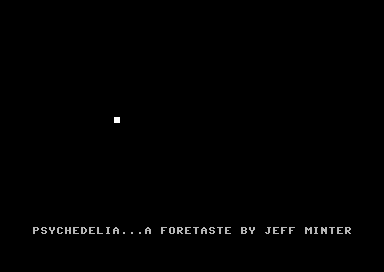
\includegraphics[height=5cm]{src/listing_commentary/foretaste.png}
  \caption*{The screen after \icode{InitializeScreenAndText} has worked its magic.}
\end{figure}

\bigskip
\bigskip
\bigskip
\bigskip
\textbf{Lines 118-132. \icode{\textbf{InitializeScreen}}:} This fills the screen with black boxes. These are the boxes we will color in each time we paint a pixel.
As mentioned before there are two components to writing a character to a screen. The first is the character
itself, the second is the color(s) of the character. Psychedelia works by drawing the same character at every
position but painting it black if its empty or filling it with color if it should be displayed. So when
we initialize the screen we paint a box at every position and paint it black.

\begin{figure}[H]
    \centering
      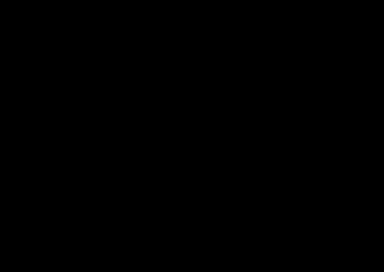
\includegraphics[height=5cm]{src/listing_commentary/black.png}
  \caption*{The screen after \icode{InitializeScreen} has painted it black.}
\end{figure}

\clearpage
\textbf{Lines 300-313. \icode{\textbf{starOneXPosArray\index{starOneXPosArray}}}}
\begin{lstlisting}[caption = Hopefully this looks familiar.,escapechar=\%]
starOneXPosArray%\index{starOneXPosArray}%
  .BYTE $00,$01,$01,$01,$00,$FF,$FF,$FF,$55       ;        5       
  .BYTE $00,$02,$00,$FE,$55                       ;                
  .BYTE $00,$03,$00,$FD,$55                       ;       4 4      
  .BYTE $00,$04,$00,$FC,$55                       ;        3       
  .BYTE $FF,$01,$05,$05,$01,$FF,$FB,$FB,$55       ;        2       
  .BYTE $00,$07,$00,$F9,$55                       ;        1       
  .BYTE $55                                       ;   4   000   4  
starOneYPosArray                                  ; 5  3210 0123  5 
  .BYTE $FF,$FF,$00,$01,$01,$01,$00,$FF,$55       ;   4   000   4  
  .BYTE $FE,$00,$02,$00,$55                       ;        1       
  .BYTE $FD,$00,$03,$00,$55                       ;        2       
  .BYTE $FC,$00,$04,$00,$55                       ;        3       
  .BYTE $FB,$FB,$FF,$01,$05,$05,$01,$FF,$55       ;       4 4      
  .BYTE $F9,$00,$07,$00,$55                       ;                
  .BYTE $55                                       ;        5       
\end{lstlisting}

\textbf{Lines 321-327. \icode{\textbf{PutRandomByteInAccumulator\index{PutRandomByteInAccumulator}}}}
\begin{lstlisting}[caption= Random\, unused\, feels like a metaphor.,escapechar=\%]
;-------------------------------------------------------
; PutRandomByteInAccumulator%\index{PutRandomByteInAccumulator}%
;-------------------------------------------------------
PutRandomByteInAccumulator%\index{PutRandomByteInAccumulator}%   
randomByteAddress=*+$01
        LDA $E199,X
        INC randomByteAddress
        RTS 
\end{lstlisting}
\textbf{Lines 434-445. \icode{\textbf{ReinitializeSequences\index{ReinitializeSequences}}}}
\begin{lstlisting}[caption = Fill our pixel arrays with zeros.,escapechar=\%]
;-------------------------------------------------------
; ReinitializeSequences%\index{ReinitializeSequences}%
;-------------------------------------------------------
ReinitializeSequences%\index{ReinitializeSequences}%   
        LDX #$00
        TXA 
ReinitializeLoop   
        STA pixelXPositionArray%\index{pixelXPositionArray}%,X
        STA pixelYPositionArray%\index{pixelYPositionArray}%,X
        STA currentColorIndexArray%\index{currentColorIndexArray}%,X
        STA initialSmoothingDelayForStep,X
        STA smoothingDelayForStep,X
        INX 
        CPX #$40
        BNE ReinitializeLoop
        RTS 

\end{lstlisting}
\clearpage

\rhead[]{\icode{starOneXPosArray\index{starOneXPosArray}/starOneYPosArray\index{starOneYPosArray}}}
\textbf{Lines 300-313. \icode{\textbf{starOneXPosArray\index{starOneXPosArray}}}:} We've encountered this data structure in our previous chapters. It encodes the pattern used in the listing as you hopefully will recall.
The commercial edition of \textit{Psychedelia} has a whole menagerie of these structures going on and we explore them in detail in
\hyperref[sec:patterns]{\textcolor{blue}{'all the pretty patterns'.}} So flick ahead there if you are impatient to find out more about them. 

\bigskip
\bigskip
\bigskip
\bigskip
\bigskip
\bigskip
\bigskip
\bigskip
\bigskip
\bigskip
\bigskip
\bigskip
\textbf{Lines 321-327.
\icode{\textbf{PutRandomByteInAccumulator\index{PutRandomByteInAccumulator}}}:}
This routine is unused in the listing but it is used by the commercial version
of 'Psychedelia': for feeding random joystick movements to the game's
attract/demo mode.  A bit of random left-over like this is not suprising when
taking the commercial source code and reducing it down for a magazine listing.

I'm obliged to point out that the routine does something very cute. The first time it is called it loads whatever is in the address \icode{\$E199} to the accumulator. That's a randomish value that can now 
be used by the caller. To ensure it produces a different number the next time it's called, it increments the \icode{\$E199} to \icode{\$E19A} before returning. Notice that
\icode{randomByteAddress} is pointing to the \icode{\$99} part of \icode{\$E199}. 

A fancier way of saying all this is that
the routine is self-mutating code! Each time it's called it increments the piece of its code that initially referenced \icode{\$E199} by calling \icode{INC randomByteAddress}. 
Thus ensuring that it always stores a new pseudo-random value in the accumulator(\icode{A}) register.

\bigskip
\textbf{Lines 434-445. \icode{\textbf{ReinitializeSequences\index{ReinitializeSequences}}}:} This is a loop that fills the 5 arrays defined on the next page with zeroes.
\icode{TXA} loads the value of \icode{\$00} previously loaded to \icode{X} to the \icode{A} register, so it could as easily be \icode{LDA \$00}
however it has the dubious advantage of being one byte shorter as an instruction.

Notice that \icode{X} gets incremented on each pass of the loop until it reaches \icode{\$40} - filling all 64 elements of each array with
\icode{\$00}.
\clearpage
\textbf{Lines 385-429. \icode{\textbf{pixelXPositionArray\index{pixelXPositionArray}}}}
\begin{lstlisting}[escapechar=\%,caption = The pixel buffers\, each 64 bytes long though only 32 bytes are used in this version thanks to \icode{MAX\_INDEX\_VALUE}
being set to \icode{\$1F} (32).]
countToMatchCurrentIndex%\index{countToMatchCurrentIndex}%      .BYTE $01
MAX_INDEX_VALUE               .BYTE $1F
pixelXPositionArray%\index{pixelXPositionArray}%   
        .BYTE $0F,$0E,$0D,$0C,$0B,$0A,$09,$04
        .BYTE $05,$06,$07,$08,$09,$0A,$0B,$0C
        .BYTE $0D,$0E,$0F,$10,$11,$12,$13,$14
        .BYTE $15,$16,$17,$14,$13,$12,$11,$10
        .BYTE $00,$00,$00,$00,$00,$00,$00,$00
        .BYTE $00,$00,$00,$00,$00,$00,$00,$00
        .BYTE $00,$00,$00,$00,$00,$00,$00,$00
        .BYTE $00,$00,$00,$00,$00,$00,$00,$00
pixelYPositionArray%\index{pixelYPositionArray}%   
        .BYTE $0C,$0D,$0E,$0F,$0F,$0F,$0E,$04
        .BYTE $04,$04,$04,$04,$04,$04,$04,$05
        .BYTE $06,$07,$08,$09,$0A,$0B,$0C,$0D
        .BYTE $0D,$0D,$0D,$07,$09,$09,$0A,$0B
        .BYTE $00,$00,$00,$00,$00,$00,$00,$00
        .BYTE $00,$00,$00,$00,$00,$00,$00,$00
        .BYTE $00,$00,$00,$00,$00,$00,$00,$00
        .BYTE $00,$00,$00,$00,$00,$00,$00,$00
currentColorIndexArray%\index{currentColorIndexArray}%   
        .BYTE $FF,$FF,$FF,$FF,$FF,$FF,$FF,$FF
        .BYTE $FF,$FF,$FF,$FF,$FF,$FF,$FF,$FF
        .BYTE $FF,$FF,$FF,$FF,$FF,$FF,$FF,$FF
        .BYTE $FF,$FF,$FF,$FF,$FF,$FF,$FF,$FF
        .BYTE $00,$00,$00,$00,$00,$00,$00,$00
        .BYTE $00,$00,$00,$00,$00,$00,$00,$00
        .BYTE $00,$00,$00,$00,$00,$00,$00,$00
        .BYTE $00,$00,$00,$00,$00,$00,$00,$00
initialSmoothingDelayForStep   
        .BYTE $0C,$0C,$0C,$0C,$0C,$0C,$0C,$0C
        .BYTE $0C,$0C,$0C,$0C,$0C,$0C,$0C,$0C
        .BYTE $0C,$0C,$0C,$0C,$0C,$0C,$0C,$0C
        .BYTE $0C,$0C,$0C,$0C,$0C,$0C,$0C,$0C
        .BYTE $00,$00,$00,$00,$00,$00,$00,$00
        .BYTE $00,$00,$00,$00,$00,$00,$00,$00
        .BYTE $00,$00,$00,$00,$00,$00,$00,$00
        .BYTE $00,$00,$00,$00,$00,$00,$00,$00
smoothingDelayForStep   
        .BYTE $04,$07,$01,$02,$03,$06,$07,$06
        .BYTE $0C,$02,$03,$06,$07,$01,$02,$02
        .BYTE $04,$04,$07,$01,$02,$03,$06,$07
        .BYTE $0C,$02,$03,$02,$03,$07,$01,$02
        .BYTE $00,$00,$00,$00,$00,$00,$00,$00
        .BYTE $00,$00,$00,$00,$00,$00,$00,$00
        .BYTE $00,$00,$00,$00,$00,$00,$00,$00
        .BYTE $00,$00,$00,$00,$00,$00,$00,$00


\end{lstlisting}
\clearpage

\rhead[]{buffer arrays}
\textbf{Lines 385-429. \icode{\textbf{pixelXPositionArray\index{pixelXPositionArray}}}:} Five arrays of 64 bytes each, though only the first 32 in each are actually used. This fact is determined
by the value of \icode{\$1F} (32) in \icode{MAX\_INDEX\_VALUE}. We see this being enforced on the next page in
\icode{MainPaintLoop\index{MainPaintLoop}}. Defining 64 bytes, but only using 32 in the end, suggests Minter\index{Minter} had to play around
with the performance limitations of the C64\index{C64}. Since each byte represents a pattern that must be drawn and painted
at a given position in the screen, using all 64 by setting allocated \icode{MAX\_INDEX\_VALUE} to \icode{\$3F} 
was not necessarily prohibitive but certainly resulted in a more sluggish effect.

We've seen the first three arrays in use already when we looked at the core
pattern painting routine. Each byte in the array refers to a distinct step in the paint sequence.
\icode{pixelXPositionArray\index{pixelXPositionArray}} and \icode{pixelYPositionArray\index{pixelYPositionArray}} together define a location on the screen
that is treated as the origin for painting and drawing an instance of the current pattern. So for example \icode{\$0F,\$0C} given by the
first byte in each represents column 16 (\icode{\$0F}) and row 14 (\icode{\$0C}). 

The value in
the corresponding position of \icode{currentColorIndexArray\index{currentColorIndexArray}} represents the color to 'start from'.

We'll cover the behaviour defined by the two 'smoothing delay' arrays in 
\hyperref[sec:dials]{\textcolor{blue}{dials buttons switches}}.
But if we look at the effect of setting this parameter to its lowest and
highest possible value below, the difference in behaviour is not
extreme. It's almost quite subtle. With a higher setting the pattern
evolves in a more drawn out fashion - as though a higher value lets
Psychedelia linger a little longer on the current state of the pattern
rather than immediately evolving it to the next state.

But we're getting ahead of ourselves, we'll come back to this behaviour in a later chapter.

\begin{figure}[H]
    \centering
    \begin{adjustbox}{width=11cm,center}
      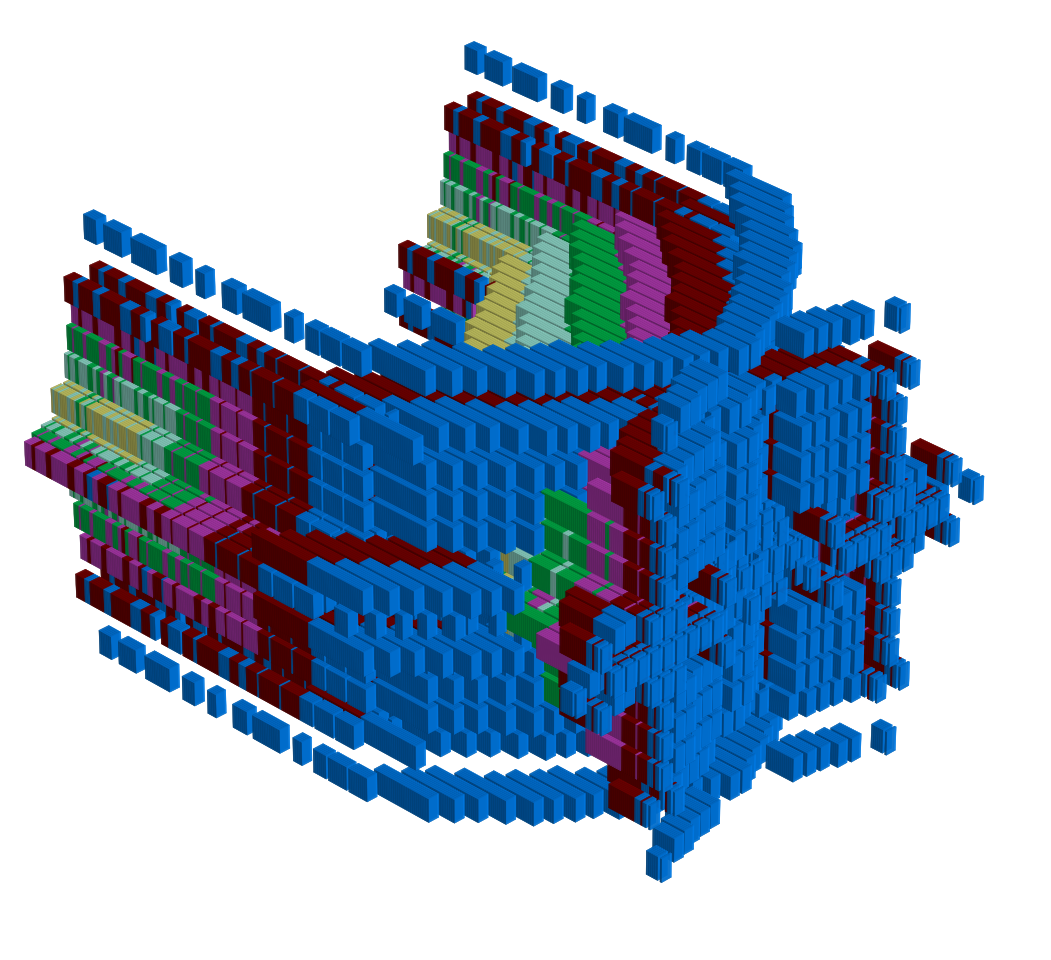
\includegraphics[width=5cm]{src/delay/pattern0-45.png}%
      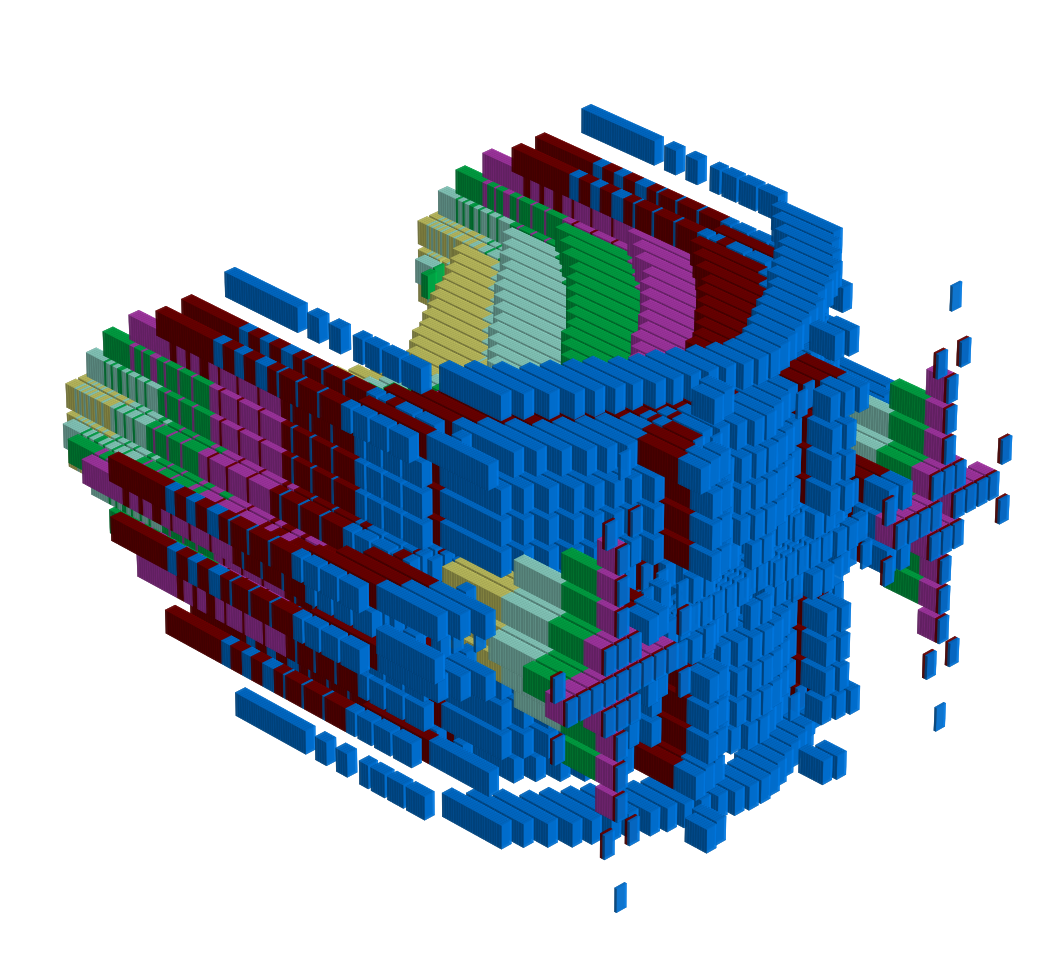
\includegraphics[width=5cm]{src/delay/pattern1-45.png}%
    \end{adjustbox}
    \caption{Effect of low and high values for Smoothing Delay}
\end{figure}



\clearpage
\textbf{Lines 450-482. \icode{\textbf{LaunchPsychedelia\index{LaunchPsychedelia}}}}
\begin{lstlisting}[caption= The game's main loop.,escapechar=\%]
;-------------------------------------------------------
; LaunchPsychedelia%\index{LaunchPsychedelia}%
;-------------------------------------------------------
LaunchPsychedelia%\index{LaunchPsychedelia}%   
        JSR ReinitializeSequences%\index{ReinitializeSequences}%
        JSR SetUpIntteruptHandler

MainPaintLoop%\index{MainPaintLoop}%   
        ; Part 1: Check if it's time to paint.
        INC currentPositionInArrays
        LDA currentPositionInArrays
        AND MAX_INDEX_VALUE
        STA currentPositionInArrays
        TAX 
        DEC smoothingDelayForStep,X
        BNE GoBackToStartOfLoop

        ; Part 2: Check if there's a color to paint.
        LDA initialSmoothingDelayForStep,X
        STA smoothingDelayForStep,X

        LDA currentColorIndexArray%\index{currentColorIndexArray}%,X
        CMP #$FF
        BEQ GoBackToStartOfLoop

        ; Part 3: Actually do a paint.
ActuallyDoAPaint
        STA currentValueInColorIndexArray%\index{currentValueInColorIndexArray}%
        LDA pixelXPositionArray%\index{pixelXPositionArray}%,X
        STA pixelXPosition%\index{pixelXPosition}%
        LDA pixelYPositionArray%\index{pixelYPositionArray}%,X
        STA pixelYPosition%\index{pixelYPosition}%

        JSR PaintStructureAtCurrentPosition%\index{PaintStructureAtCurrentPosition}%

        LDX currentPositionInArrays
        DEC currentColorIndexArray%\index{currentColorIndexArray}%,X

GoBackToStartOfLoop   
        JMP MainPaintLoop%\index{MainPaintLoop}%

\end{lstlisting}

\begin{figure}[H]
  {
    \setlength{\tabcolsep}{3.0pt}
    \setlength\cmidrulewidth{\heavyrulewidth} % Make cmidrule = 
    \begin{adjustbox}{width=7cm,center}

      \begin{tabular}{rllllllll}
        \toprule
        Byte & Bit 7 & Bit 6 & Bit 5 & Bit 4 & Bit 3 & Bit 2 & Bit 1 & Bit 0        \\
        \midrule
        \$20 & 0 & 0 & 1 & 0 & 0 & 0 & 0 & 0 \\
        \$1F & 0 & 0 & 0 & 1 & 1 & 1 & 1 & 1 \\
        \midrule
        Result & 0 & 0 & 0 & 0 & 0 & 0 & 0 & 0 \\
        \addlinespace
        \bottomrule
      \end{tabular}
    \end{adjustbox}
    }\caption*{AND'ing \$20 and \$1F gives \$00, ensuring we always loop between 0 and 32.}
\end{figure}
\clearpage
\rhead[]{\icode{LaunchPsychedelia\index{LaunchPsychedelia}}}
\textbf{Lines 450-482. \icode{\textbf{LaunchPsychedelia\index{LaunchPsychedelia}}}:} Finally a routine that resembles getting down to business. We start by initializing the arrays we saw on the 
previous page to all zeros in \icode{ReinitializeSequences\index{ReinitializeSequences}}. Next we set up the interrupt handler, which will
be responsible for processing user input. We'll take a look at this routine in more detail later on.

For now, what follows is the game's core loop. This runs forever, round and round, repeating all the steps between the
\icode{MainPaintLoop\index{MainPaintLoop}} and \icode{GoBackToStartOfLoop} labels. 

There are three parts to the code inside this loop. 

The first is visited on every journey through the loop and increments the
value stored in \icode{currentPositionInArrays}. It keeps this value looping between 0 and 32 by always \icode{AND}'ing
it with \icode{MAX\_INDEX\_VALUE}. 

\begin{lstlisting}
        LDA currentPositionInArrays
        AND MAX_INDEX_VALUE
        STA currentPositionInArrays
\end{lstlisting}

This \icode{AND} operation ensures that once it reaches 33, for example, the result
goes back to zero. (See opposite page.)

Now that it has a new value in \icode{currentPositionInArrays} it transfers it to the \icode{X} register and uses the 
\icode{X} as in index into the \icode{smoothingDelayForStep} array (and all the other arrays) which we saw defined on the previous 
page. It decrements the byte at this index in the \icode{smoothingDelayForStep} array and if it has reached zero
proceeds to Part 2 of the loop, otherwise it jumps execution to \icode{GoBackToStartOfLoop}, which itself jumps execution
back to the top again at \icode{MainPaintLoop\index{MainPaintLoop}}. Back on the merry-go-round we go.

If we get to Part 2 this time round we first reset the value in the \icode{framesRemaining\-ToNextPaintForStep} array with an initial value for it kept in the corresponding
location of \icode{initialFramesRemaining\-ToNextPaintForStep}. We next check if we've run out of colors to paint for this step
in the sequence: if the value at the index position in \icode{currentColorIndexArray\index{currentColorIndexArray}} has already reached \icode{\$FF} (because
it was decremented below zero and so cycled back to \icode{\$FF}) then there's nothing to paint and we jump back to the top
again via \icode{GoBackToStartOfLoop}. No colors means no painting after all!

If there actually, finally, is something to do for this position in the sequence we can pass to Part 3. Here we load up the X and Y
position to use from our \icode{pixelXPositionArray\index{pixelXPositionArray}} and \icode{pixelYPositionArray\index{pixelYPositionArray}} and do the actual painting work we covered
in our previous chapter, all of which happens in \icode{PaintStructureAtCurrentPosition\index{PaintStructureAtCurrentPosition}}. As we saw this routine is the top of the
tree for the pixel painting routines in Psychedelia, and all it needed from us here was an X and Y position as well as a color
loaded from the \icode{currentColorIndexArray\index{currentColorIndexArray}}. Equipped with that it can paint anything. 

\clearpage
\textbf{Lines 217-285. \icode{\textbf{PaintStructureAtCurrentPosition\index{PaintStructureAtCurrentPosition}}}}
\begin{lstlisting}[caption = The routine responsible for orchestrating the pattern painting.,escapechar=\%]
NUM_ARRAYS = $07
;-------------------------------------------------------
; PaintStructureAtCurrentPosition%\index{PaintStructureAtCurrentPosition}%
;-------------------------------------------------------
PaintStructureAtCurrentPosition%\index{PaintStructureAtCurrentPosition}%   
        JSR PaintPixelForCurrentSymmetry%\index{PaintPixelForCurrentSymmetry}%

        LDY #$00
        LDA currentValueInColorIndexArray%\index{currentValueInColorIndexArray}%
        CMP #NUM_ARRAYS
        BNE CanLoopAndPaint
        RTS 

CanLoopAndPaint   
        LDA #NUM_ARRAYS
        STA countToMatchCurrentIndex%\index{countToMatchCurrentIndex}%
       
        LDA pixelXPosition%\index{pixelXPosition}%
        STA initialPixelXPosition
        LDA pixelYPosition%\index{pixelYPosition}%
        STA initialPixelYPosition

LineReadLoop   
        ; See next page for the contents of this loop.
        JMP LineReadLoop

RestorePositionsAndReturn%\index{RestorePositionsAndReturn}%   
        LDA initialPixelXPosition
        STA pixelXPosition%\index{pixelXPosition}%
        LDA initialPixelYPosition
        STA pixelYPosition%\index{pixelYPosition}%
        RTS 

\end{lstlisting}
\clearpage

\rhead[]{\icode{PaintStructureAtCurrentPosition\index{PaintStructureAtCurrentPosition}}}
\textbf{Lines 217-285. \icode{\textbf{PaintStructureAtCurrentPosition\index{PaintStructureAtCurrentPosition}}}:} To understand how this routine and the ones it calls on the subsequent pages hang together you should refer
back to the previous chapter 
\hyperref[sec:listing_pattern]{\textcolor{blue}{'soul of a small light machine'.}} 
Here we will limit ourselves to explaining some of the detailed points of the code.

The meat of this routine occurs in the \icode{LineReadLoop} section on the next page but here we can see the
gatekeeping and bookkeeping activities of the code before and after that central section. 

The first call to \icode{PaintPixelForCurrentSymmetry\index{PaintPixelForCurrentSymmetry}} paints a pixel at the current position given by 
\icode{pixelXPosition\index{pixelXPosition}} and \icode{pixelYPosition\index{pixelYPosition}}. The \icode{-CurrentSymmetry} part ensures that extra
pixels are projected along the axes given by the current symmetry setting. In our listing this is the
X-axis, ensuring we always paint two patterns. We'll look at this in a little more detail later.

Next we figure out if we should just return early from this routine and do nothing further. This will be the
case if \icode{currentValueInColorIndexArray\index{currentValueInColorIndexArray}} is still at the same value as \icode{NUM\_ARRAYS} (7). If it is
we return from the routine straight away (\icode{RTS}) and
\icode{MainPaintLoop\index{MainPaintLoop}} will decrement it the next time around for this position
in the sequence and we can paint an actual color.

You cans see that before and after the \icode{LineReadLoop} section we're storing the values in \icode{pixelX/YPosition} in
\icode{initialPixelX/YPosition} and then restoring them when the loop is over. This is because \icode{LineReadLoop}
will frequently overwrite the values as it iterates through the positions given in the pattern array \icode{starOneX/YPosArray}.

\vspace{2cm}

\begin{definition2}[Friendly Blue Learning Box: \icode{CMP}]
\setlength{\intextsep}{0pt}%
\setlength{\columnsep}{3pt}%
\small
\icode{CMP} compares the value given as an argument with the value in the \icode{A} and returns a 1 if they match and a zero if they
  do not. So if we have loaded \icode{\$02} to \icode{A} and do \icode{CMP \#NUM\_ARRAYS} (where \icode{NUM\_ARRAYS = \$07}) it will return a zero,
  as they do not match. Our subsequent statement \icode{BNE CanLoopAndPaint} inspects this result: if they are not equal execution will
  jump to \icode{CanLoopAndPaint} otherwise it will continue on to \icode{RTS} and return from the routine without doing anything further.
\end{definition2}
\clearpage
\textbf{Lines 239-278. \icode{\textbf{LineReadLoop}}}
\begin{lstlisting}[caption=The core pattern-painting loop.,escapechar=\%]
LineReadLoop   
        LDA initialPixelXPosition
        CLC 
        ADC starOneXPosArray%\index{starOneXPosArray}%,Y
        STA pixelXPosition%\index{pixelXPosition}%

        LDA initialPixelYPosition
        CLC 
        ADC starOneYPosArray%\index{starOneYPosArray}%,Y
        STA pixelYPosition%\index{pixelYPosition}%

        TYA 
        PHA 

        JSR PaintPixelForCurrentSymmetry%\index{PaintPixelForCurrentSymmetry}%

        PLA 
        TAY 
        INY 

        LDA starOneXPosArray%\index{starOneXPosArray}%,Y
        CMP #$55
        BNE LineReadLoop

        DEC countToMatchCurrentIndex%\index{countToMatchCurrentIndex}%
        LDA countToMatchCurrentIndex%\index{countToMatchCurrentIndex}%
        CMP currentValueInColorIndexArray%\index{currentValueInColorIndexArray}%
        BEQ RestorePositionsAndReturn%\index{RestorePositionsAndReturn}%
        CMP #$01
        BEQ RestorePositionsAndReturn%\index{RestorePositionsAndReturn}%

        INY 
        JMP LineReadLoop

\end{lstlisting}
\begin{lstlisting}[escapechar=\%]
starOneXPosArray%\index{starOneXPosArray}%
  .BYTE $00,$01,$01,$01,$00,$FF,$FF,$FF,$55       ;        5       
  .BYTE $00,$02,$00,$FE,$55                       ;                
  .BYTE $00,$03,$00,$FD,$55                       ;       4 4      
  .BYTE $00,$04,$00,$FC,$55                       ;        3       
  .BYTE $FF,$01,$05,$05,$01,$FF,$FB,$FB,$55       ;        2       
  .BYTE $00,$07,$00,$F9,$55                       ;        1       
  .BYTE $55                                       ;   4   000   4  
starOneYPosArray%\index{starOneYPosArray}%                                  ; 5  3210 0123  5
  .BYTE $FF,$FF,$00,$01,$01,$01,$00,$FF,$55       ;   4   000   4  
  .BYTE $FE,$00,$02,$00,$55                       ;        1       
  .BYTE $FD,$00,$03,$00,$55                       ;        2       
  .BYTE $FC,$00,$04,$00,$55                       ;        3       
  .BYTE $FB,$FB,$FF,$01,$05,$05,$01,$FF,$55       ;       4 4      
  .BYTE $F9,$00,$07,$00,$55                       ;                
  .BYTE $55                                       ;        5       
                                                  
\end{lstlisting}
\clearpage

\rhead[]{\icode{PaintStructureAtCurrentPosition\index{PaintStructureAtCurrentPosition}: LineReadLoop}}
\textbf{Lines 239-278. \icode{\textbf{LineReadLoop}}:} A better name for this loop might be \icode{ThisIsWhereThe\-PsychedeliaHappens}. As I keep saying (if only you would listen), we unpicked the mechanics
of the \icode{Paint\-StructureAtCurrentPosition} routine that this loop is a
part of in the previous chapter
\hyperref[sec:listing_pattern]{\textcolor{blue}{'soul of a small light machine'.}} 
This littlw routine reads off lines from our pattern data structure and paints them to the screen by calling \icode{PaintPixelForCurrentSymmetry}. 
it doesn't do them all at once of course. The number of lines it reads off and converts to stages of the pattern on the screen is controlled by \icode{currentValueInColorIndexArray}. So let's take a look at how it works.

Our index into the pattern array is stored in \icode{Y}, this is what will enable us to read in the data in each line and detect the segment breaks in the pattern given by \icode{\$55}
. \icode{Y} starts out at zero and gets incremented at
each pass through the loop. So the first paragraph adds the value at index 0 in \icode{starOneXPosArray\index{starOneXPosArray}} in this pass to \icode{initialPixelXPosition}
and stores it in \icode{pixelXPosition\index{pixelXPosition}}. That value is \icode{\$00}, on the next it will be \icode{\$01}, on the pass after that
it will be \icode{\$01} again, as these are the values it is reading from the array. You can hopefully see how the \icode{LDA}, \icode{ADC}, and \icode{STA} instructions are doing that
but you might wonder what the \icode{CLC} is about. This clears the CPU's 'Carry Bit' so that the addition performed by \icode{ADC}
doesn't inadvertently include any carries from previous addition operations in its result.

The next paragraph does the same for \icode{pixelYPosition\index{pixelYPosition}} using the \icode{starOneXPosArray\index{starOneXPosArray}} array. But the paragraph after
that does something that requires explanation. It transfers the current value in the \icode{Y} register to the \icode{A} register
using the instruction \icode{TYA}. Then it pushes the \icode{A} register on to a thing called the 'Stack' using the instruction
\icode{PHA}. The 'Stack' is a stack of values that resembles a stack of plates: you add things to the top of it and take things
from the top of it. So when you take something from the stack using the complementary instruction \icode{PLA} you are taking
what was last put there (and not pulled off it before you).

So the \icode{TYA, PHA, PLA, TAY} sequence of instructions that surrounds our call to \icode{PaintPixelForCurrentSymmetry\index{PaintPixelForCurrentSymmetry}} has the
simple effect of ensuring that we keep our current value of \icode{Y} unmolested by whatever \icode{PaintPixelForCurrentSymmetry\index{PaintPixelForCurrentSymmetry}}
gets up to, because that can (and does) include populating and using the \icode{Y} register for other stuff. As you can imagine
this is a common technique in a CPU where there are only three free variables to play with (\icode{X,Y,A}) and you have more than three things
to worry about!

Next, after incrementing \icode{Y} (\icode{INY}) we check the next value in \icode{starOneXPosArray\index{starOneXPosArray}}. If it's \icode{\$55} then
we've reached the end of a line the pattern and must check whether we've read all the lines in the pattern we need to for this
round. If we have, then we return by calling \icode{RestorePositionsAndReturn\index{RestorePositionsAndReturn}}, otherwise we increment \icode{Y} again to read
in the first value of the next line and continue looping.

\clearpage
\textbf{Lines 332-382. \icode{\textbf{PaintPixelForCurrentSymmetry\index{PaintPixelForCurrentSymmetry}}}}
\begin{lstlisting}[caption=Choosing what to paint based on the current symmetry setting.,escapechar=\%]
currentSymmetrySettingForStep%\index{currentSymmetrySettingForStep}%   .BYTE $01

PaintPixelForCurrentSymmetry%\index{PaintPixelForCurrentSymmetry}%   
        ; First paint the normal pattern without any
        ; symmetry.
        LDA pixelXPosition%\index{pixelXPosition}%
        PHA 
        LDA pixelYPosition%\index{pixelYPosition}%
        PHA 
        JSR PaintPixel%\index{PaintPixel}%

        LDA currentSymmetrySettingForStep%\index{currentSymmetrySettingForStep}%
        BNE HasSymmetry

CleanUpAndReturnFromSymmetry   
        PLA 
        STA pixelYPosition%\index{pixelYPosition}%
        PLA 
        STA pixelXPosition%\index{pixelXPosition}%
        RTS 

HasSymmetry   
        ; Has a pattern to paint on the X axis
        ; symmetry so prepare for that.
        LDA #NUM_COLS
        SEC 
        SBC pixelXPosition%\index{pixelXPosition}%
        STA pixelXPosition%\index{pixelXPosition}%

        JSR PaintPixel%\index{PaintPixel}%

        LDA currentSymmetrySettingForStep%\index{currentSymmetrySettingForStep}%
        CMP #$01
        BEQ CleanUpAndReturnFromSymmetry

        LDA #NUM_ROWS
        SEC 
        SBC pixelYPosition%\index{pixelYPosition}%
        STA pixelYPosition%\index{pixelYPosition}%
        JSR PaintPixel%\index{PaintPixel}%

        PLA 
        TAY 
        PLA 
        STA pixelXPosition%\index{pixelXPosition}%
        TYA 
        PHA 
        JSR PaintPixel%\index{PaintPixel}%
        PLA 
        STA pixelYPosition%\index{pixelYPosition}%
        RTS 

\end{lstlisting}
\clearpage

\rhead[]{\icode{PaintPixelForCurrentSymmetry\index{PaintPixelForCurrentSymmetry}}}
\textbf{Lines 332-382. \icode{\textbf{PaintPixelForCurrentSymmetry\index{PaintPixelForCurrentSymmetry}}}:} This routine is concerned entirely with setting up the values of \icode{pixelXPosition\index{pixelXPosition}} and \icode{pixelYPosition\index{pixelYPosition}} correctly
for calling the routine \icode{PaintPixel\index{PaintPixel}}. The reason this is necessary is that the commercial version of Psychedelia
has up to 4 different arrangements or 'symmetries' for painting the chosen pattern. The simplest arrangement is just to 
paint one copy of the pattern and be done. The first paragraph here takes care of that, no matter what arrangement we're
painting we're always painting the pattern at least once. 

While the commercial version has at least three others to worry about, and offers the user a way of switching between each,
the listing edition hard-codes a single behaviour of always painting the pattern twice, reflected on the X-axis in a kind of mirror
arrangement. This behaviour is defined by the value in \icode{currentSymmetrySettingForStep\index{currentSymmetrySettingForStep}} and as we can see opposite it
is hard-coded to \icode{\$01}. Because it is set to a non-zero value, \icode{BNE HasSymmetry} always returns true and execution
jumps to \icode{HasSymmetry}.

\icode{HasSymmetry} calculates the reflected position on the X-axis for the pattern by simply subtracting the current value
of \icode{pixelXPosition\index{pixelXPosition}} from the total number of columns in the screen (which is 40). This has the neat effect of ensuring
the reflected position is always exactly opposite to the original pattern.

The paragraph after \icode{PaintPixel\index{PaintPixel}} always returns from the routine because as we saw \icode{currentSymmetrySettingForStep\index{currentSymmetrySettingForStep}} is
hardcoded to \icode{\$01}. So the code after it is never executed and is redundant here. What it does is draw a full four-pattern
arrangement with reflections along the X and Y axes. If we set \icode{currentSymmetrySettingForStep\index{currentSymmetrySettingForStep}} to \icode{\$02} and run the
listing we can see this in action.


\begin{figure}[H]
    \centering
      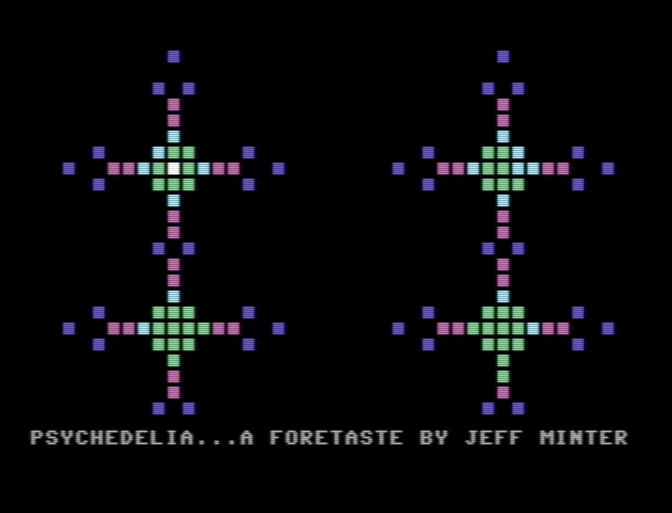
\includegraphics[height=5cm]{src/listing_commentary/four_pattern.png}
  \caption*{The display with \icode{currentSymmetrySettingForStep\index{currentSymmetrySettingForStep}} set to \icode{\$02}}
\end{figure}


\clearpage
\textbf{Lines 164-214. \icode{\textbf{PaintPixel\index{PaintPixel}}}}
\begin{lstlisting}[caption=Where the painting is actually done.,escapechar=\%]
presetColorValuesArray%\index{presetColorValuesArray}%
;         0    6    2    4      5    3     7      1
  .BYTE BLACK,BLUE,RED,PURPLE,GREEN,CYAN,YELLOW,WHITE
;-------------------------------------------------------
; PaintPixel%\index{PaintPixel}%
;-------------------------------------------------------
PaintPixel%\index{PaintPixel}%   
        LDA pixelXPosition%\index{pixelXPosition}%
        AND #$80 ; Detect if has moved off left of screen
        BNE ReturnEarly
        LDA pixelXPosition%\index{pixelXPosition}%
        CMP #NUM_COLS
        BPL ReturnEarly
        LDA pixelYPosition%\index{pixelYPosition}%
        AND #$80 ; Detect if has moved off top of screen.
        BNE ReturnEarly
        LDA pixelYPosition%\index{pixelYPosition}%
        CMP #NUM_ROWS
        BPL ReturnEarly

        JSR LoadXAndYPosition%\index{LoadXAndYPosition}%
        LDA (currentLineForPixelInColorRamLoPtr),Y
        AND #COLOR_MAX

        LDX #$00
CheckPresetsLoop   
        CMP presetColorValuesArray%\index{presetColorValuesArray}%,X
        BEQ MaybePaintPixel
        INX 
        CPX #COLOR_MAX + 1
        BNE CheckPresetsLoop

MaybePaintPixel   
        TXA 
        STA indexOfCurrentColor%\index{indexOfCurrentColor}%
        LDX currentValueInColorIndexArray%\index{currentValueInColorIndexArray}%
        INX 
        CPX indexOfCurrentColor%\index{indexOfCurrentColor}%
        BEQ ActuallyPaintPixel%\index{ActuallyPaintPixel}%
        BPL ActuallyPaintPixel%\index{ActuallyPaintPixel}%
        RTS 

ActuallyPaintPixel%\index{ActuallyPaintPixel}%   
        LDX currentValueInColorIndexArray%\index{currentValueInColorIndexArray}%
        LDA presetColorValuesArray%\index{presetColorValuesArray}%,X
        STA (currentLineForPixelInColorRamLoPtr),Y
        RTS 
\end{lstlisting}
\clearpage

\rhead[]{\icode{PaintPixel\index{PaintPixel}}}
\textbf{Lines 164-214. \icode{\textbf{PaintPixel\index{PaintPixel}}}:} The first paragraph searches for a reason to \icode{ReturnEarly}. The first
check, whether the pixel has moved beyond the leftmost position on the screen, is a good example of how assembly language involves
logic that might be unintuitive at first. In layman's terms we just want to ask is \icode{pixelXPosition\index{pixelXPosition}} less than zero. One neat
way of doing this in our situation is to check if decrementing past \icode{\$00} has resulted in a value of \icode{\$FF} (Decrementing zero 'wraps
around' to \icode{\$FF}). Since
the rightmost position never exceeds \icode{\$40} this means we can just check if the leftmost bit on the value is set or not: if 
it is then we've gone below zero. So an \icode{AND \$80} check will do the job - if it returns true then we've gone below zero:

\begin{figure}[H]
  {
    \setlength{\tabcolsep}{3.0pt}
    \setlength\cmidrulewidth{\heavyrulewidth} % Make cmidrule = 
    \begin{adjustbox}{width=7cm,center}

      \begin{tabular}{rllllllll}
        \toprule
        Byte & Bit 7 & Bit 6 & Bit 5 & Bit 4 & Bit 3 & Bit 2 & Bit 1 & Bit 0        \\
        \midrule
        \$FF & 1 & 1 & 1 & 1 & 1 & 1 & 1 & 1 \\
        \$80 & 1 & 0 & 0 & 0 & 0 & 0 & 0 & 0 \\
        \midrule
        Result & 1 & 0 & 0 & 0 & 0 & 0 & 0 & 0 \\
        \addlinespace
        \bottomrule
      \end{tabular}
    \end{adjustbox}
    }\caption*{AND'ing \$FF and \$80 gives \$80, a non-zero value - so the \icode{AND} returns true.}
\end{figure}

If we get past these checks we can prepare ourselves for writing to the screen by calling \icode{LoadXAndYPosition\index{LoadXAndYPosition}}. As we can
see below this loads the \icode{Y} position to the \icode{X} register and the \icode{X} position to the \icode{Y} register. There
is a reason that this is what seems like the wrong way round - the use we intend to make of each register is constrained by the
rules of assembly language. 

\begin{lstlisting}[escapechar=\%]
LoadXAndYPosition%\index{LoadXAndYPosition}%   
        LDX pixelYPosition%\index{pixelYPosition}%
        LDA colorRAMLineTableLoPtrArray%\index{colorRAMLineTableLoPtrArray}%,X
        STA currentLineForPixelInColorRamLoPtr
        LDA colorRAMLineTableHiPtrArray%\index{colorRAMLineTableHiPtrArray}%,X
        STA currentLineForPixelInColorRamHiPtr
        LDY pixelXPosition%\index{pixelXPosition}%
        RTS 
\end{lstlisting}
Both \icode{X} and \icode{Y} can be used as offsets when referencing addresses in memory, but the specific use
we need to make of each means that we cannot store our X position in \icode{X} and our \icode{Y} position in Y, which is a shame!

\textbf{Lines 210-214. \icode{\textbf{ActuallyPaintPixel\index{ActuallyPaintPixel}}}:} This is the rubber hitting the road. We're writing data to the
screen. Recall that our  \icode{colorRAMLineTableLoPtrArray\index{colorRAMLineTableLoPtrArray}} array is an array of 25 screen addresses each one pointing
to the start of a row. In \icode{LoadXAndYPosition\index{LoadXAndYPosition}} we have set up \icode{currentLineForPixelInColorRamLoPtr} and \icode{currentLine\-ForPixelInColorRamHiPtr} to contain the address of the pixel we want to paint. So for example if the address of Color RAM we want to populate
is \icode{\$D810} then \icode{currentLineForPixelInColorRamLoPtr} will contain \icode{\$10} and \icode{currentLine\-ForPixelInColorRamHiPtr} will
contain \icode{\$D8}. 
\clearpage
\textbf{Lines 491-506. \icode{\textbf{SetUpInterruptHandler}}}
\begin{lstlisting}[caption= Setting up our Interrupt Handler,escapechar=\%]
SetUpIntteruptHandler   
        SEI 
        LDA #<MainInterruptHandler
        STA $0314    ;IRQ
        LDA #>MainInterruptHandler
        STA $0315    ;IRQ

        LDA #$0A
        STA cursorXPosition%\index{cursorXPosition}%
        STA cursorYPosition%\index{cursorYPosition}%

        LDA #$01
        STA $D015    ;Sprite display Enable
        STA $D027    ;Sprite 0 Color
        CLI 
        RTS 
\end{lstlisting}
\clearpage
\rhead[]{\icode{SetUpInterruptHandler}}
\textbf{Lines 491-506. \icode{\textbf{SetUpInterruptHandler}}:} What is an Interrupt Handler when it's at home and why are
we setting one up?

Recall that this routine was called immediately before we entered the main loop. It is only ever called once:
\begin{lstlisting}[escapechar=\%]
LaunchPsychedelia%\index{LaunchPsychedelia}%   
        JSR ReinitializeSequences%\index{ReinitializeSequences}%
        JSR SetUpIntteruptHandler
\end{lstlisting}

In plain English, an 'interrupt' is when the CPU periodically stops what ever its doing and does some other pre-defined amount
of work instead. There are a few such interrupts supported by the 6502 CPU but the one we make use of here is called the IRQ
or 'Hardware Interrupt'. This interrupt runs 60 times a second (that's right, 60 times a second) and already has some work
assigned to it by the Commodore 64, a set of tasks such as checking keyboard and joystick input that is defined at address \icode{\$EA31}.
This doesn't have a proper name of it's own so we will call it \icode{DEFAULT\_IRQ\_HANDLER}. (The routine called by an interrupt
is often referred to as an 'interrupt vector'.)

What we can do is tag some work of our own onto this, we still need to call the routine at \icode{\$EA31} but we can do some of our
own stuff before it. The way to do this is to load the address of our own routine, which we call \icode{MainInterruptHandler}, to
the address that the 6502 CPU consults each time it interrupts its work. We replace \icode{\$EA31} at that address with the address
of \icode{MainInterruptHandler}.  
\begin{lstlisting}[escapechar=\%]
        SEI 
        LDA #<MainInterruptHandler
        STA $0314    ;IRQ
        LDA #>MainInterruptHandler
        STA $0315    ;IRQ
        ...
        CLI 
\end{lstlisting}

Notice that because the address is two bytes long we must split it out, like we did for our Colour RAM address earlier, into 
two bytes and store each one separate in the consecutive address locations \icode{\$0314} and \icode{\$0315}, which store
the second and first byte of the interrupt-handler address respectively. 

The \icode{SEI} instruction at the beginning of this routine and the \icode{CLI} instruction at the end tell the CPU that we 
are updating the interrupt vector. The \icode{SEI} ensures that no further interrupts happen while we are doing this, and the
\icode{CLI} gives the CPU the all-clear to start honouring interrupts again now that we've updated the routine it should call
when one happens.


\clearpage
\textbf{Lines 491-506. \icode{\textbf{MainInterruptHandler}}}
\begin{lstlisting}[caption= This is our interrupt handler\, it runs 60 times a second so has to be fast.,escapechar=\%]
MainInterruptHandler   
        DEC countStepsBeforeCheckingJoystickInput%\index{countStepsBeforeCheckingJoystickInput}%
        BEQ PaintCursorAndCheckJoystickInput
        JMP DEFAULT_IRQ_HANDLER

PaintCursorAndCheckJoystickInput   
        LDA #$02
        STA countStepsBeforeCheckingJoystickInput%\index{countStepsBeforeCheckingJoystickInput}%
        LDA #$00
        STA currentColorToPaint%\index{currentColorToPaint}%
        JSR PaintCursorAtCurrentPosition%\index{PaintCursorAtCurrentPosition}%

CheckIfJoystickMovedUpOrDown   
        LDA $DC00    ;CIA1: Data Port Register A
        AND #$03
        CMP #$03
        BEQ CheckIfPlayerPressedLeftOrRight

        CMP #$02
        BEQ PlayerHasPressedDown

PlayerHasPressedUp
        ; Player has pressed up. Incremeent up two lines
        ; so that when we decrement down one, we're still
        ; one up!
        INC cursorYPosition%\index{cursorYPosition}%
        INC cursorYPosition%\index{cursorYPosition}%

PlayerHasPressedDown   
        DEC cursorYPosition%\index{cursorYPosition}%
        LDA cursorYPosition%\index{cursorYPosition}%
        CMP #$FF
        BNE CheckIfCursorAtBottom

WrapCursorToBottom
        ; Cursor has reached the top of the screen, so loop
        ; around to bottom.
        LDA #NUM_ROWS - 1
        STA cursorYPosition%\index{cursorYPosition}%
        JMP CheckIfPlayerPressedLeftOrRight

CheckIfCursorAtBottom   
        CMP #NUM_ROWS
        BNE CheckIfPlayerPressedLeftOrRight
        ; Cursor has reached the bottom of the screen, so loop
        ; around to top
        LDA #$00
        STA cursorYPosition%\index{cursorYPosition}%

\end{lstlisting}
\clearpage

\rhead[]{\icode{MainInterruptHandler}}
\textbf{Lines 491-506. \icode{\textbf{MainInterruptHandler}}:}  You don't have to look too hard at our interrupt handler
to divine what is is mainly concerned with: have you moved the joystick or pressed fire? The routine is long enough
that we need to spread it over 3 pages here. The section on the opposite page gets as far as reacting to any up or
down movement in the joystick and the beginnings of the left/right checks. 

Joystick input is read from the \icode{CIA1 Data Port Register}. If the player interacts with the joystick at all it will
show up in the byte at address \icode{\$DC00}. Only 5 of the 8 bits are used, 4 for each direction and 1 for the fire button.
Counter-intuitively, the bits are set to \icode{1} by default, so you can tell if a button has been pressed or the joystick moved
if one of the appropriate bits is \icode{0} rather than \icode{1}.

\begin{figure}[H]
  {
    \setlength{\tabcolsep}{3.0pt}
    \setlength\cmidrulewidth{\heavyrulewidth} % Make cmidrule = 
    \begin{adjustbox}{width=7cm,center}

      \begin{tabular}{rllllllll}
        \toprule
        Byte & Bit 7 & Bit 6 & Bit 5 & Bit 4 & Bit 3 & Bit 2 & Bit 1 & Bit 0        \\
             &       &       &       & Fire  & Right & Left  & Down  & Up           \\
        \midrule
        \$FD & 1 & 1 & 1 & 1 & 1 & 1 & 0 & 1 \\
        \bottomrule
      \end{tabular}
    \end{adjustbox}
  }\caption*{The contents of \icode{\$DC00} when the player has pressed down on the joystick.}
\end{figure}

\textbf{Lines 491-506. \icode{\textbf{CheckIfJoystickMovedUpOrDown}}:} If we \icode{AND} the value in \icode{\$DC00} (for
example, \icode{\$FE}) with
\icode{\$03} it will tell us if up or down have been pressed if the result is not equal to \icode{\$03}. This is because
we expect both bits to be 1 if up or down have not been pressed, and the \icode{AND} ensures we are only comparing those
two bits when we perform \icode{CMP \#\$03}.
\begin{figure}[H]
  {
    \setlength{\tabcolsep}{3.0pt}
    \setlength\cmidrulewidth{\heavyrulewidth} % Make cmidrule = 
    \begin{adjustbox}{width=7cm,center}

      \begin{tabular}{rllllllll}
        \toprule
        Byte & Bit 7 & Bit 6 & Bit 5 & Bit 4 & Bit 3 & Bit 2 & Bit 1 & Bit 0        \\
             &       &       &       & Fire  & Right & Left  & Down  & Up           \\
        \midrule
        \$FE & 1 & 1 & 1 & 1 & 1 & 1 & 1 & 0 \\
        \$03 & 0 & 0 & 0 & 0 & 0 & 0 & 1 & 1 \\
        \midrule
        Result & 0 & 0 & 0 & 0 & 0 & 0 & 1 & 0 \\
        \addlinespace
        \bottomrule
      \end{tabular}
    \end{adjustbox}
    }\caption*{AND'ing \$FE and \$03 gives \$02, telling us that 'Up' has been pressed.}
\end{figure}

Once we have established this we can increment and decrement \icode{cursorYPosition\index{cursorYPosition}} as appropriate and also check
if we've reached the top or bottom of the screen. 
\clearpage
\textbf{Lines 300-313. \icode{\textbf{CheckIfPlayerPressedLeftOrRight}}}
\begin{lstlisting}[caption= Second part of the Interrupt Handler.,escapechar=\%]
CheckIfPlayerPressedLeftOrRight   
        LDA $DC00    ;CIA1: Data Port Register A
        AND #$0C
        CMP #$0C
        BEQ CheckIfPlayerPressedFire%\index{CheckIfPlayerPressedFire}%

        CMP #$08
        BEQ PlayerHasPressedLeft

PlayerHasPressedRight
        ; Player has pressed right.
        INC cursorXPosition%\index{cursorXPosition}%
        INC cursorXPosition%\index{cursorXPosition}%

PlayerHasPressedLeft   
        DEC cursorXPosition%\index{cursorXPosition}%
        LDA cursorXPosition%\index{cursorXPosition}%
        CMP #$FF
        BNE CheckIfCursorAtExtremeRight

WrapCursorToExtremeRight
        LDA #NUM_COLS - 1
        STA cursorXPosition%\index{cursorXPosition}%
        JMP CheckIfPlayerPressedFire%\index{CheckIfPlayerPressedFire}%

CheckIfCursorAtExtremeRight   
        CMP #NUM_COLS
        BNE CheckIfPlayerPressedFire%\index{CheckIfPlayerPressedFire}%
        LDA #$00
        STA cursorXPosition%\index{cursorXPosition}%

\end{lstlisting}
\clearpage
\rhead[]{\icode{MainInterruptHandler} cont.}
\textbf{Lines 300-313. \icode{\textbf{CheckIfPlayerPressedLeftOrRight}}:} As in the previous page, which was checking
for up/down movement, here we're checking for left/right movement in the joystick and updating the \icode{cursorXPosition\index{cursorXPosition}} if required.

\begin{figure}[H]
  {
    \setlength{\tabcolsep}{3.0pt}
    \setlength\cmidrulewidth{\heavyrulewidth} % Make cmidrule = 
    \begin{adjustbox}{width=7cm,center}

      \begin{tabular}{rllllllll}
        \toprule
        Byte & Bit 7 & Bit 6 & Bit 5 & Bit 4 & Bit 3 & Bit 2 & Bit 1 & Bit 0        \\
             &       &       &       & Fire  & Right & Left  & Down  & Up           \\
        \midrule
        \$F7 & 1 & 1 & 1 & 1 & 0 & 1 & 1 & 1 \\
        \$0C & 0 & 0 & 0 & 0 & 1 & 1 & 0 & 0 \\
        \midrule
        Result & 0 & 0 & 0 & 0 & 0 & 1 & 0 & 0 \\
        \addlinespace
        \bottomrule
      \end{tabular}
    \end{adjustbox}
    }\caption*{AND'ing \$F7 and \$0C gives \$04, telling us that 'Left' has been pressed.}
\end{figure}

\clearpage
\textbf{Lines 300-313. \icode{\textbf{CheckIfPlayerPressedFire\index{CheckIfPlayerPressedFire}}}}
\begin{lstlisting}[caption= Third part of the Interrupt Handler.,escapechar=\%]
CheckIfPlayerPressedFire%\index{CheckIfPlayerPressedFire}%   
        LDA $DC00    ;CIA1: Data Port Register A
        AND #$10
        BEQ PlayerHasPressedFire

PlayerHasntPressedFire
        LDA #$00
        STA stepsSincePressedFire%\index{stepsSincePressedFire}%
        JMP DrawCursorAndReturnFromInterrupt%\index{DrawCursorAndReturnFromInterrupt}%

PlayerHasPressedFire
MaybeUpdatePixelBuffers   
        LDA unusedBurstMode
        BEQ UpdateArrayIndex

        LDA stepsSincePressedFire%\index{stepsSincePressedFire}%
        BNE DrawCursorAndReturnFromInterrupt%\index{DrawCursorAndReturnFromInterrupt}%
        INC stepsSincePressedFire%\index{stepsSincePressedFire}%

UpdateArrayIndex   
        INC indexIntoArrays
        LDA indexIntoArrays
        AND MAX_INDEX_VALUE
        STA indexIntoArrays

CheckCurrentIndexInBuffers  
        TAX 
        LDA currentColorIndexArray%\index{currentColorIndexArray}%,X
        CMP #$FF
        BNE DrawCursorAndReturnFromInterrupt%\index{DrawCursorAndReturnFromInterrupt}%

UpdateBuffersWithCursorPosition
        LDA cursorXPosition%\index{cursorXPosition}%
        STA pixelXPositionArray%\index{pixelXPositionArray}%,X
        LDA cursorYPosition%\index{cursorYPosition}%
        STA pixelYPositionArray%\index{pixelYPositionArray}%,X
        LDA #COLOR_MAX
        STA currentColorIndexArray%\index{currentColorIndexArray}%,X

        LDA smoothingDelay%\index{smoothingDelay}%
        STA initialSmoothingDelayForStep,X
        STA smoothingDelayForStep,X

\end{lstlisting}
\clearpage

\rhead[]{\icode{MainInterruptHandler} cont.}
\textbf{Lines 300-313. \icode{\textbf{CheckIfPlayerPressedFire\index{CheckIfPlayerPressedFire}}}:} This section of the routine could be much shorter. This
is because neither \icode{burstModeEnabled} nor \icode{stepsSincePressedFire\index{stepsSincePressedFire}} are actually used. The code that refers
to them seems to be concerned with supporting an unused feature toggled on/off by the variable \icode{burstModeEnabled}
and since it has been hardcoded to \icode{\$00} the section could be stripped back to this instead:

\begin{lstlisting}[escapechar=\%]
CheckIfPlayerPressedFire%\index{CheckIfPlayerPressedFire}%   
        LDA $DC00    ;CIA1: Data Port Register A
        AND #$10
        BNE DrawCursorAndReturnFromInterrupt%\index{DrawCursorAndReturnFromInterrupt}%

PlayerHasPressedFire
        INC indexIntoArrays
        LDA indexIntoArrays
        AND MAX_INDEX_VALUE
        STA indexIntoArrays

CheckCurrentIndexInBuffers  
        TAX 
        LDA currentColorIndexArray%\index{currentColorIndexArray}%,X
        CMP #$FF
        BNE DrawCursorAndReturnFromInterrupt%\index{DrawCursorAndReturnFromInterrupt}%

UpdateBuffersWithCursorPosition
        LDA cursorXPosition%\index{cursorXPosition}%
        STA pixelXPositionArray%\index{pixelXPositionArray}%,X
        LDA cursorYPosition%\index{cursorYPosition}%
        STA pixelYPositionArray%\index{pixelYPositionArray}%,X
        LDA #COLOR_MAX
        STA currentColorIndexArray%\index{currentColorIndexArray}%,X

        LDA smoothingDelay%\index{smoothingDelay}%
        STA initialSmoothingDelayForStep,X
        STA smoothingDelayForStep,X
\end{lstlisting}

This refactored version makes it much easier to see what's going on: if the player has pressed fire then we increment
our index into the pixel arrays and load the cursor's position to the index's position in \icode{pixelXPositionArray\index{pixelXPositionArray}/pixelYPositionArray\index{pixelYPositionArray}}
and initial values to the arrays managing pixel color and smoothing delay.

If the player hasn't pressed fire or if our current index to the arrays points to a position that is already being used then
we skip to just painting the cursor and exiting. Note that our heuristic for deciding whether the current position in the 
arrays is in use is to make sure that the value at \icode{indexIntoArrays} in \icode{currentColorIndexArray\index{currentColorIndexArray}} is \icode{\$FF} - 
after all, this will only be the case if we haven't already used it (or used it up).

\clearpage
\textbf{Lines 300-313. \icode{\textbf{DrawCursorAndReturnFromInterrupt\index{DrawCursorAndReturnFromInterrupt}}}}
\begin{lstlisting}[caption = Paint the cursor and call the system default interrupt handler \icode{RETURN\_FROM\_INTERRUPT},escapechar=\%]
DrawCursorAndReturnFromInterrupt%\index{DrawCursorAndReturnFromInterrupt}%   
        JSR LoadXAndYOfCursorPosition%\index{LoadXAndYOfCursorPosition}%
        LDA (currentLineForCursorInColorRamLoPtr),Y
        AND #COLOR_MAX
        STA lastColorPainted
        LDA #WHITE
        STA currentColorToPaint%\index{currentColorToPaint}%
        JSR PaintCursorAtCurrentPosition%\index{PaintCursorAtCurrentPosition}%
        JMP RETURN_FROM_INTERRUPT

\end{lstlisting}

\bigskip
\textbf{Lines 300-313. \icode{\textbf{LoadXAndYOfCursorPosition\index{LoadXAndYOfCursorPosition}}}}
\begin{lstlisting}[escapechar=\%][caption= Load the X and Y position and set up \icode{currentLineForCursorInColorRamLoPtr/currentLineForCursorInColorRamHiPtr}[escapechar=\%]
for painting the cursor.]
LoadXAndYOfCursorPosition%\index{LoadXAndYOfCursorPosition}%   
        LDX cursorYPosition%\index{cursorYPosition}%
        LDA colorRAMLineTableLoPtrArray%\index{colorRAMLineTableLoPtrArray}%,X
        STA currentLineForCursorInColorRamLoPtr
        LDA colorRAMLineTableHiPtrArray%\index{colorRAMLineTableHiPtrArray}%,X
        STA currentLineForCursorInColorRamHiPtr
        LDY cursorXPosition%\index{cursorXPosition}%
        RTS 
\end{lstlisting}
\bigskip
\textbf{Lines 300-313. \icode{\textbf{PaintCursorAtCurrentPosition\index{PaintCursorAtCurrentPosition}}}}
\begin{lstlisting}[caption = Paint the cursor.,escapechar=\%]
PaintCursorAtCurrentPosition%\index{PaintCursorAtCurrentPosition}%   
        JSR LoadXAndYOfCursorPosition%\index{LoadXAndYOfCursorPosition}%
        LDA currentColorToPaint%\index{currentColorToPaint}%
        STA (currentLineForCursorInColorRamLoPtr),Y
        RTS 
\end{lstlisting}
\clearpage

\rhead[]{\icode{DrawCursorAndReturnFromInterrupt\index{DrawCursorAndReturnFromInterrupt}}}
\textbf{Lines 300-313. \icode{\textbf{DrawCursorAndReturnFromInterrupt\index{DrawCursorAndReturnFromInterrupt}}}:} Drawing the cursor should be a relatively simple matter
of converting the cursor position stored in \icode{cursorXPosition\index{cursorXPosition}} and \icode{cursorYPosition\index{cursorYPosition}} to a position on the screen. Again
we have some redundant code to distract us: there is no good reason to determine the \icode{lastColorPainted} since we don't use it
for anything (and this code is not present in the commercial edition). So our simplified version of \icode{DrawCursor\-AndReturnFromInterrupt}
looks as follows:
\begin{lstlisting}[escapechar=\%]
DrawCursorAndReturnFromInterrupt%\index{DrawCursorAndReturnFromInterrupt}%   
        JSR LoadXAndYOfCursorPosition%\index{LoadXAndYOfCursorPosition}%
        LDA #WHITE
        STA currentColorToPaint%\index{currentColorToPaint}%
        JSR PaintCursorAtCurrentPosition%\index{PaintCursorAtCurrentPosition}%
        JMP RETURN_FROM_INTERRUPT
\end{lstlisting}

The real work is clearly done by our two helper routines \icode{LoadXAndYOfCursorPosition\index{LoadXAndYOfCursorPosition}} and \icode{PaintCursorAtCurrentPosition\index{PaintCursorAtCurrentPosition}}. 

Let's imagine our cursor has an \icode{cursorYPosition\index{cursorYPosition}} of 5 and an \icode{cursorXPosition\index{cursorXPosition}} of 10. This means in \icode{LoadXAndYOfCursorPosition\index{LoadXAndYOfCursorPosition}}
we will retrieve the elements with index 5 in \icode{colorRAMLineTableLoPtrArray\index{colorRAMLineTableLoPtrArray}} and \icode{colorRAMLineTableHiPtrArray\index{colorRAMLineTableHiPtrArray}}. So consulting
our table below we see the values we end up with in each highlighted in red:

\begin{figure}[H]
  {
    \setlength{\tabcolsep}{3.0pt}
    \setlength\cmidrulewidth{\heavyrulewidth} % Make cmidrule = 
    \begin{adjustbox}{width=8cm,center}
      \begin{tabular}{cccc}
        \toprule
        Element &
        \makecell[c]{\icode{colorRAMLineTable} \\ \icode{HiPtrArray}} & 
        \makecell[c]{\icode{colorRAMLineTable} \\ \icode{LoPtrArray}} & 
        Address \\
        \midrule
0 & \icode{\$D8} & \icode{\$00} & \icode{\$D800} \\ 
1 & \icode{\$D8} & \icode{\$28} & \icode{\$D828} \\ 
2 & \icode{\$D8} & \icode{\$50} & \icode{\$D850} \\ 
3 & \icode{\$D8} & \icode{\$78} & \icode{\$D878} \\ 
4 & \icode{\$D8} & \icode{\$A0} & \icode{\$D8A0} \\ 
        \textcolor{red}{5} & \textcolor{red}{\icode{\$D8}} & \textcolor{red}{\icode{\$C8}} & \textcolor{red}{\icode{\$D8C8}} \\ 
        \bottomrule
      \end{tabular}
    \end{adjustbox}
  }
\end{figure}
\vspace*{-\baselineskip}

With an address of \icode{\$D8C8} we now know where in Color RAM our line starts. We can now load our \icode{cursorXPosition\index{cursorXPosition}} to the
\icode{Y} register:
\begin{lstlisting}[escapechar=\%]
        LDY cursorXPosition%\index{cursorXPosition}%
\end{lstlisting}
And use that to paint the cursor position white. The address we want to paint is \icode{(currentLineForCursorInColorRamLoPtr)} + 
\icode{Y}, i.e. \icode{\$D8C8} + \icode{\$0A} = \icode{\$D8D2}. We express this in assembly as follows:
\begin{lstlisting}[escapechar=\%]
        LDA currentColorToPaint%\index{currentColorToPaint}%
        STA (currentLineForCursorInColorRamLoPtr),Y
\end{lstlisting}






